% Options for packages loaded elsewhere
\PassOptionsToPackage{unicode}{hyperref}
\PassOptionsToPackage{hyphens}{url}
%
\documentclass[
  a4paper]{article}
\usepackage{lmodern}
\usepackage{amssymb,amsmath}
\usepackage{ifxetex,ifluatex}
\ifnum 0\ifxetex 1\fi\ifluatex 1\fi=0 % if pdftex
  \usepackage[T1]{fontenc}
  \usepackage[utf8]{inputenc}
  \usepackage{textcomp} % provide euro and other symbols
\else % if luatex or xetex
  \usepackage{unicode-math}
  \defaultfontfeatures{Scale=MatchLowercase}
  \defaultfontfeatures[\rmfamily]{Ligatures=TeX,Scale=1}
  \setsansfont[]{Calibri Light}
\fi
% Use upquote if available, for straight quotes in verbatim environments
\IfFileExists{upquote.sty}{\usepackage{upquote}}{}
\IfFileExists{microtype.sty}{% use microtype if available
  \usepackage[]{microtype}
  \UseMicrotypeSet[protrusion]{basicmath} % disable protrusion for tt fonts
}{}
\makeatletter
\@ifundefined{KOMAClassName}{% if non-KOMA class
  \IfFileExists{parskip.sty}{%
    \usepackage{parskip}
  }{% else
    \setlength{\parindent}{0pt}
    \setlength{\parskip}{6pt plus 2pt minus 1pt}}
}{% if KOMA class
  \KOMAoptions{parskip=half}}
\makeatother
\usepackage{xcolor}
\IfFileExists{xurl.sty}{\usepackage{xurl}}{} % add URL line breaks if available
\IfFileExists{bookmark.sty}{\usepackage{bookmark}}{\usepackage{hyperref}}
\hypersetup{
  hidelinks,
  pdfcreator={LaTeX via pandoc}}
\urlstyle{same} % disable monospaced font for URLs
\usepackage[margin=1in]{geometry}
\usepackage{graphicx,grffile}
\makeatletter
\def\maxwidth{\ifdim\Gin@nat@width>\linewidth\linewidth\else\Gin@nat@width\fi}
\def\maxheight{\ifdim\Gin@nat@height>\textheight\textheight\else\Gin@nat@height\fi}
\makeatother
% Scale images if necessary, so that they will not overflow the page
% margins by default, and it is still possible to overwrite the defaults
% using explicit options in \includegraphics[width, height, ...]{}
\setkeys{Gin}{width=\maxwidth,height=\maxheight,keepaspectratio}
% Set default figure placement to htbp
\makeatletter
\def\fps@figure{htbp}
\makeatother
\setlength{\emergencystretch}{3em} % prevent overfull lines
\providecommand{\tightlist}{%
  \setlength{\itemsep}{0pt}\setlength{\parskip}{0pt}}
\setcounter{secnumdepth}{-\maxdimen} % remove section numbering
\usepackage{fancyhdr}
\usepackage[T1]{fontenc}
\usepackage[default]{sourcesanspro}
\usepackage{tikz}
\addtolength{\headheight}{1.0cm} 
\fancypagestyle{plain}{} 
\thispagestyle{fancy} 
\renewcommand{\headrulewidth}{0pt}

% Package for references with numbers
\bibliographystyle{apsrev4-1}
\usepackage[numbers]{natbib}
\setcitestyle{numbers}
\usepackage[brazil]{babel}
\usepackage{amsmath}
\usepackage{titling}

\usepackage{background}

\backgroundsetup{
position={3,0.55},
scale=1.2,
color=black,
opacity=1,
angle=0,
pages=all,
contents={%
  
\includegraphics[width=200px,height=200px]{Imagens/logo_header.jpg}
  }%
}
\usepackage{floatrow}
\floatsetup[figure]{capposition=top}
\floatsetup[table]{capposition=top}


\usepackage{fancyhdr}
\pagestyle{fancy}
% center of header
\fancyhf{} % clear all header and footer fields

\renewcommand{\headrulewidth}{0pt}
\usepackage{booktabs}
\usepackage{longtable}
\usepackage{array}
\usepackage{multirow}
\usepackage{wrapfig}
\usepackage{float}
\usepackage{colortbl}
\usepackage{pdflscape}
\usepackage{tabu}
\usepackage{threeparttable}
\usepackage{threeparttablex}
\usepackage[normalem]{ulem}
\usepackage{makecell}
\usepackage{xcolor}

\author{}
\date{\vspace{-2.5em}}

\begin{document}

\rhead{\fontsize{8pt}{10pt} \selectfont Núcleo de Segurança do Paciente
\\ \fontsize{8pt}{10pt} \selectfont Centro Nacional de Controle de Qualidade

}

\begin{center}
 {\LARGE Programa Primeiro Estágio}
\end{center}
\vspace{0cm}

\subsection{PROTOCOLO DE IDENTIFICAÇÃO DO PACIENTE}

\begin{figure}[H]
\caption{Percentual de pacientes com pulseiras padronizadas entre os pacientes avaliados}
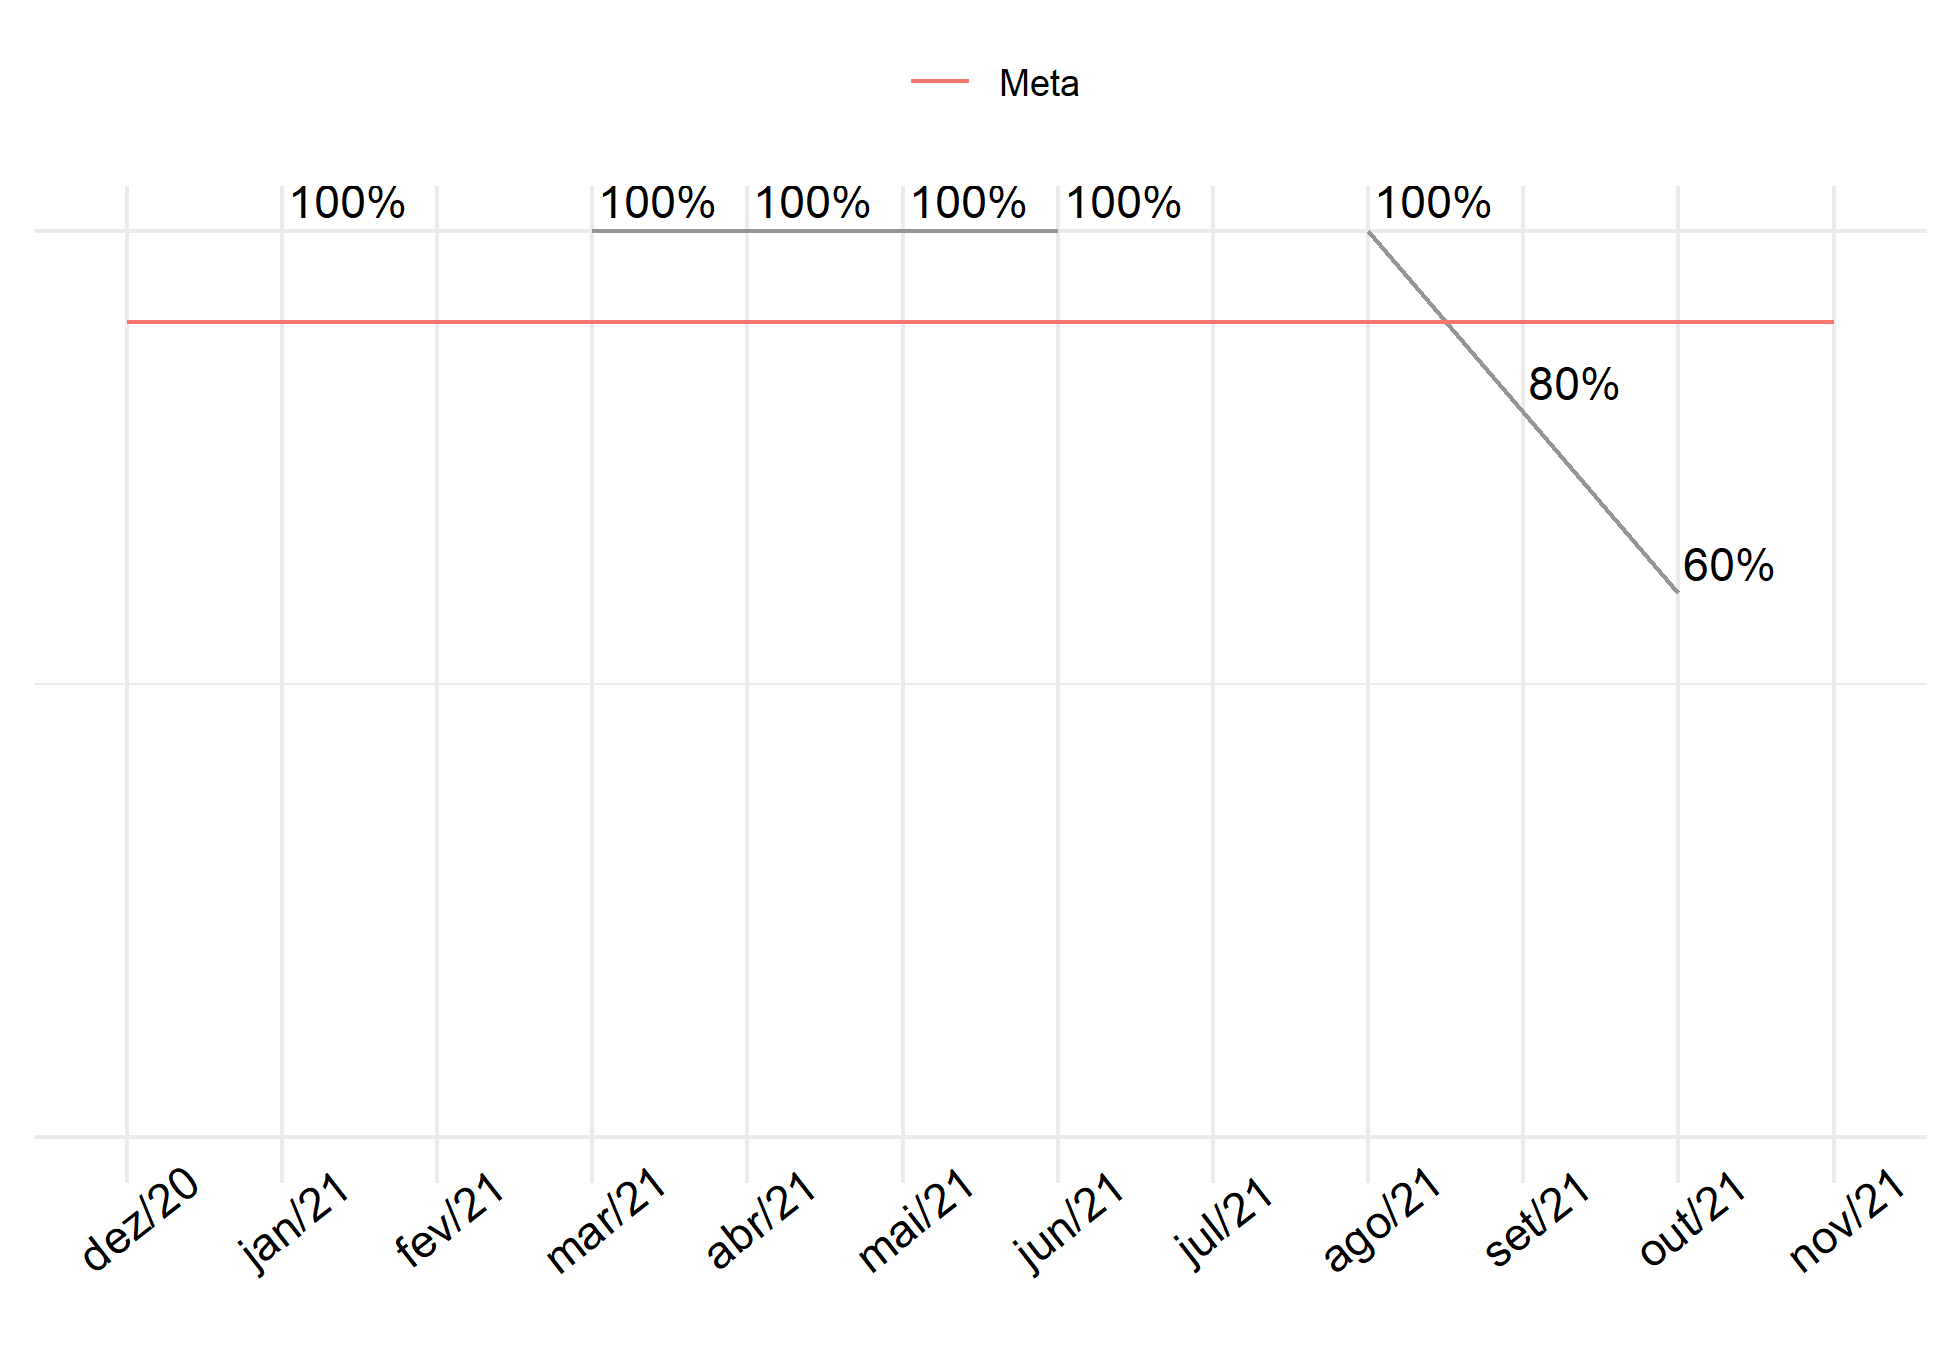
\includegraphics[width=0.7\textwidth]{Imagens/pulseiras.png}
\end{figure}

\begin{center}
 \textbf{Meta: 90\%}
\end{center}

\begin{figure}[H]
\caption{Proporção de criados identificados entre os criados observados}
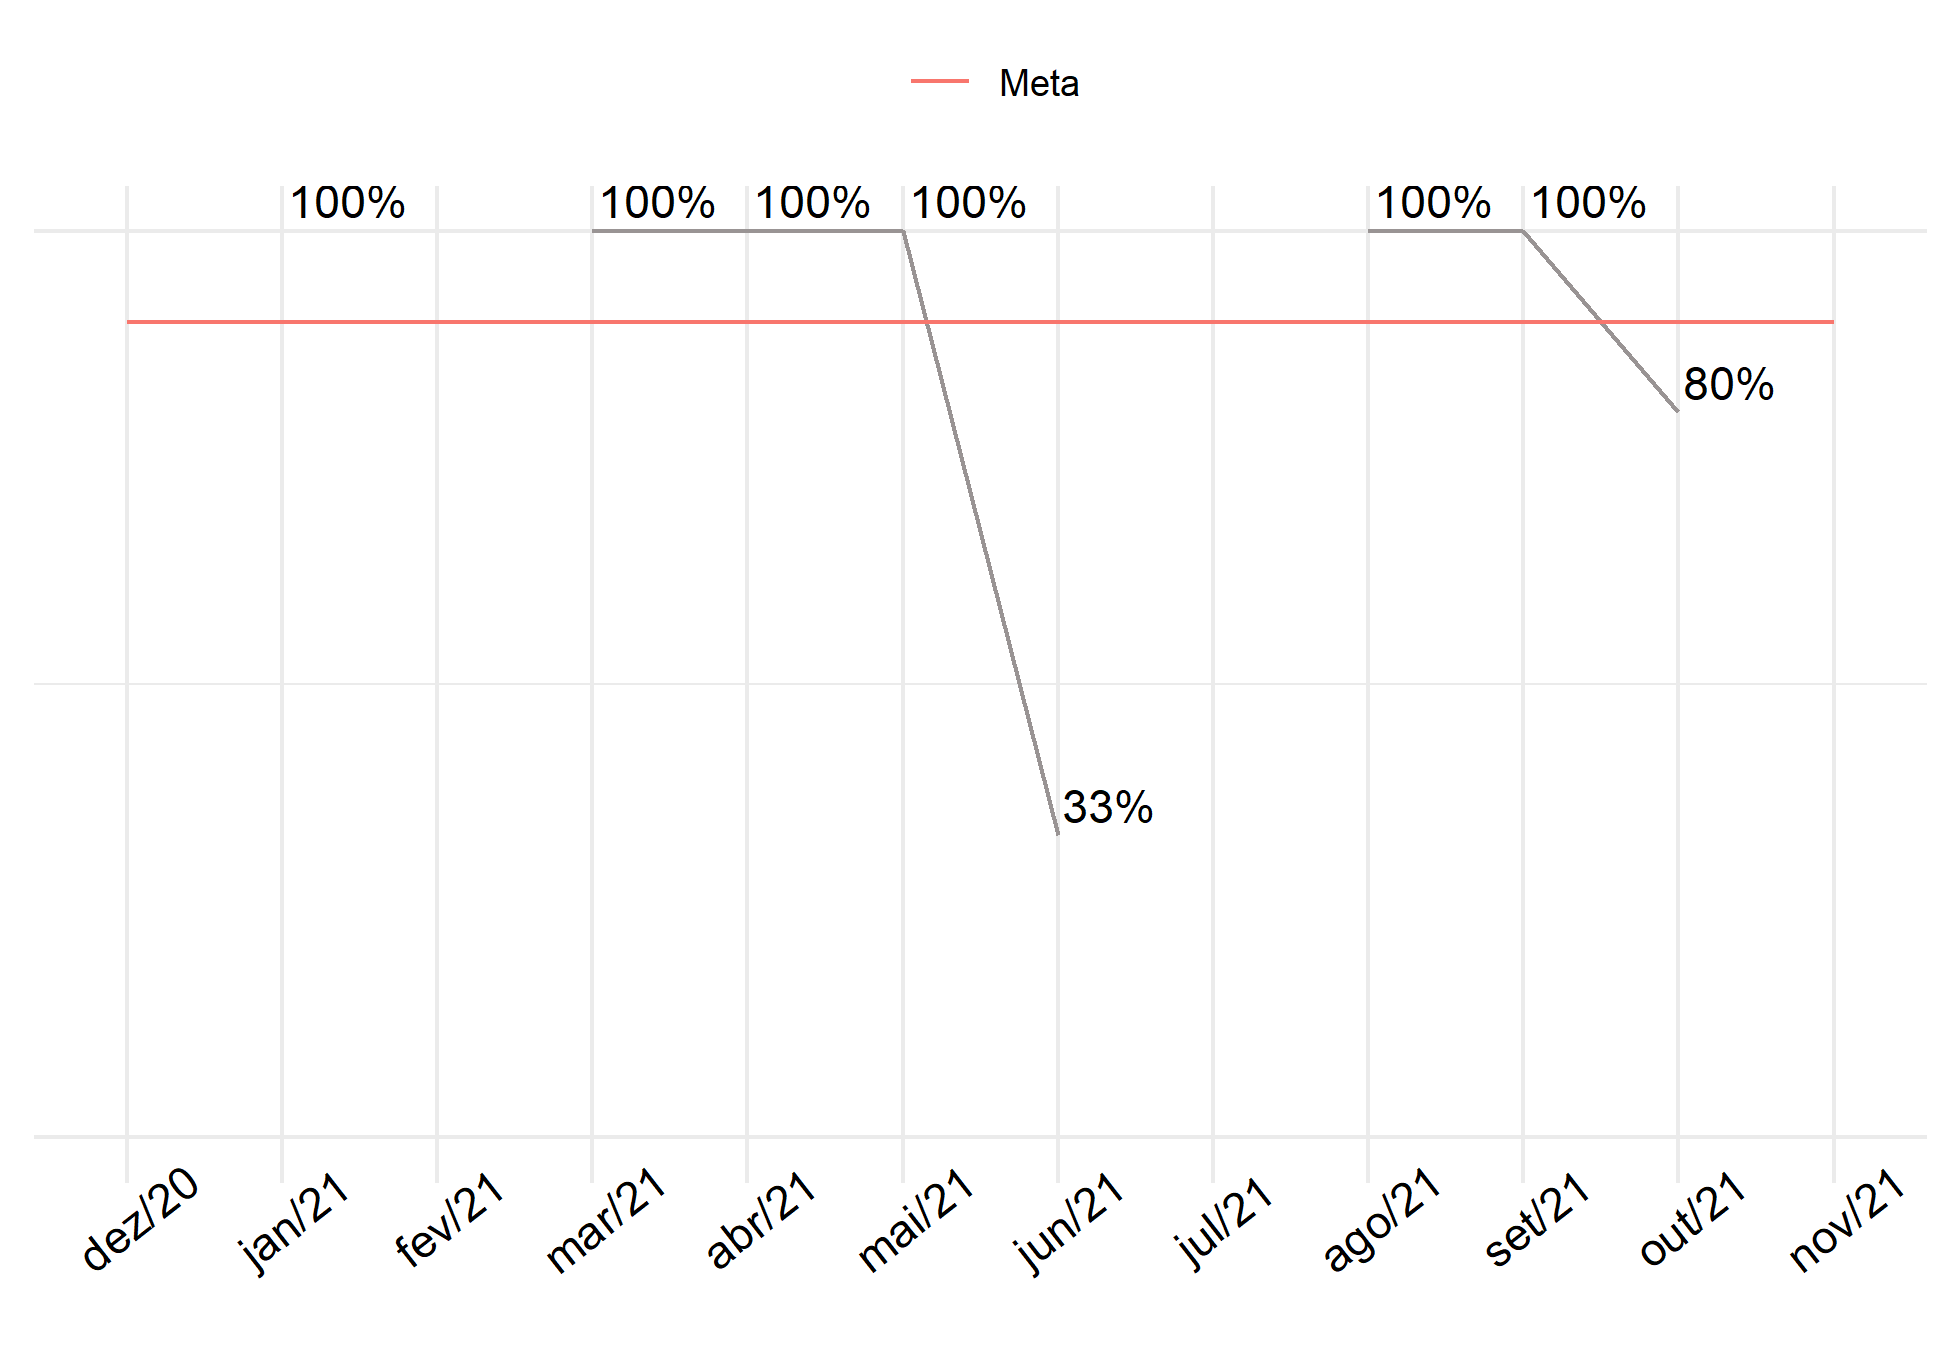
\includegraphics[width=0.7\textwidth]{Imagens/criado.png}
\end{figure}

\begin{center}
 \textbf{Meta: 100\%}
\end{center}

\begin{figure}[H]
\caption{Proporção de cama-macas identificadas entre as cama-macas observadas}
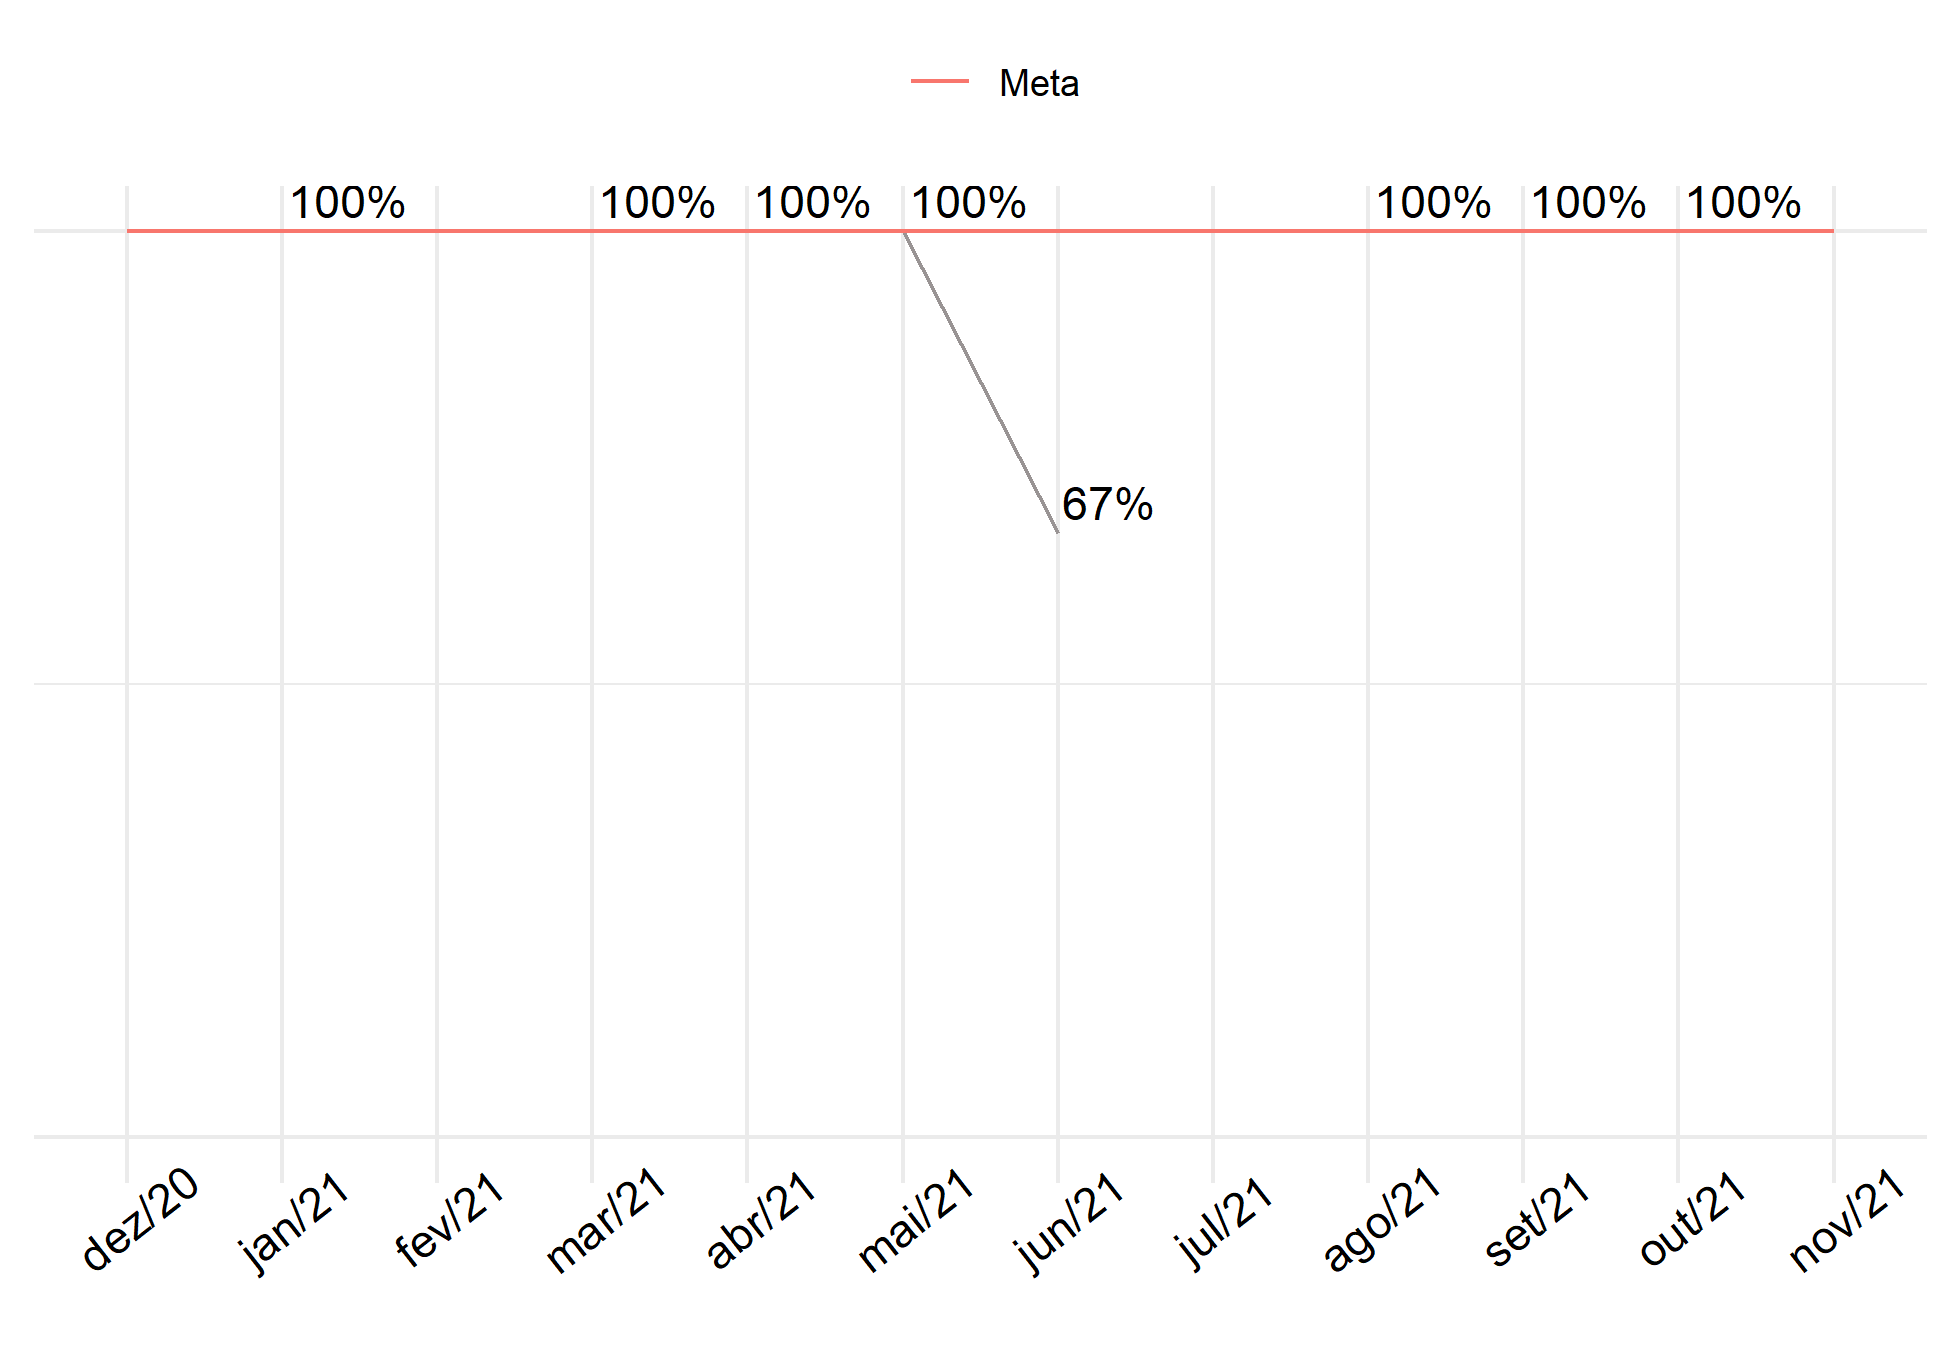
\includegraphics[width=0.7\textwidth]{Imagens/cama.png}
\end{figure}

\begin{center}
 \textbf{Meta: 100\%}
\end{center}

\subsection{COMUNICAÇÃO SEGURA}

\begin{figure}[H]
\caption{Percentual de preenchimento do check list de comunicação segura à admissão}
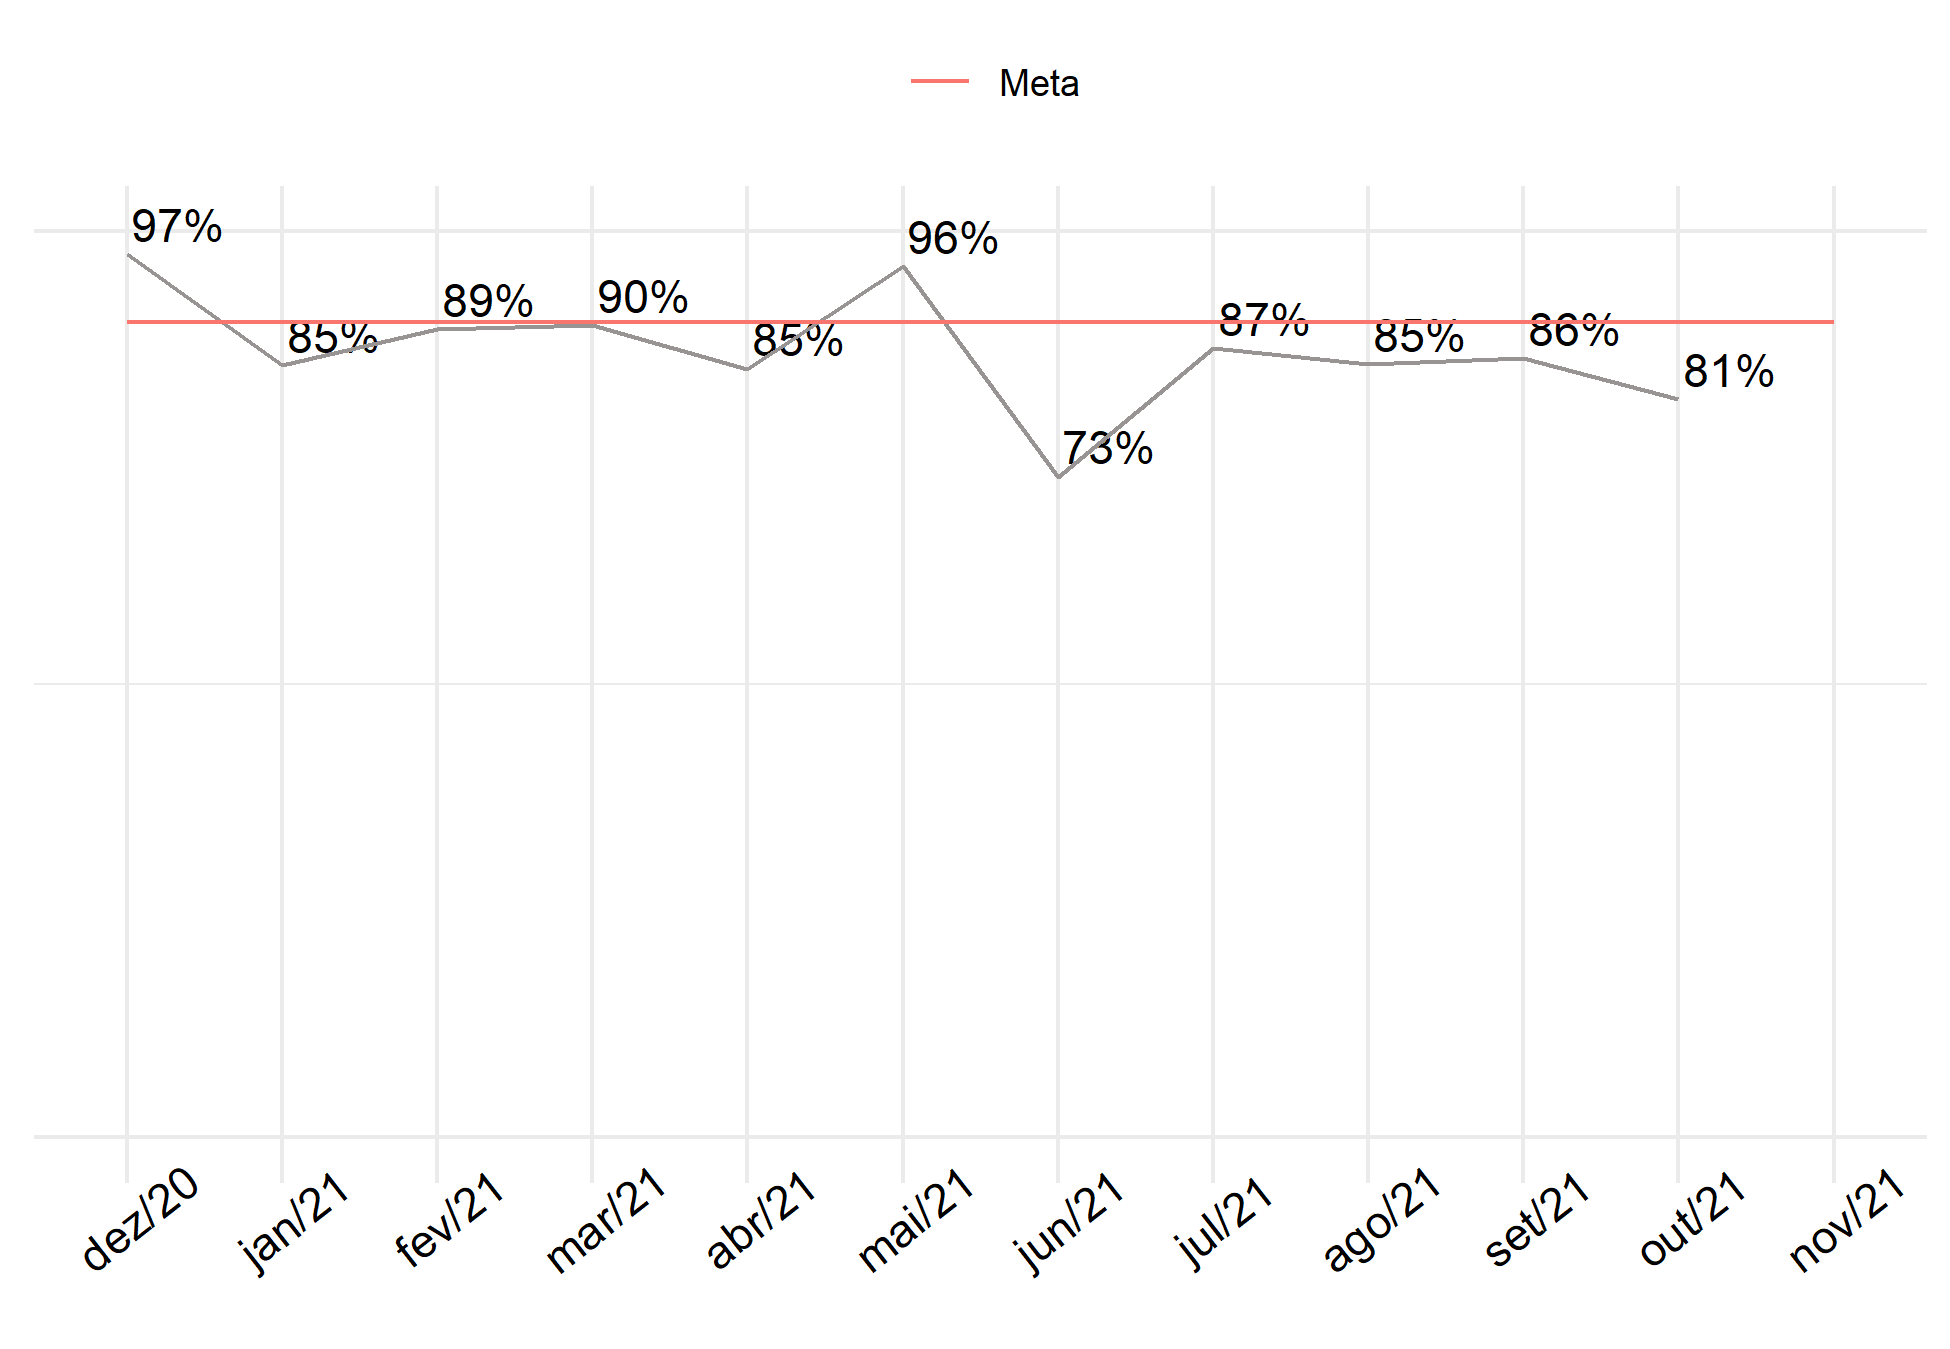
\includegraphics[width=0.7\textwidth]{Imagens/check_admissao.png}
\end{figure}

\begin{center}
 \textbf{Meta: 90\%}
\end{center}

\begin{figure}[H]
\caption{Percentual de preenchimento do check list de comunicação segura na alta}
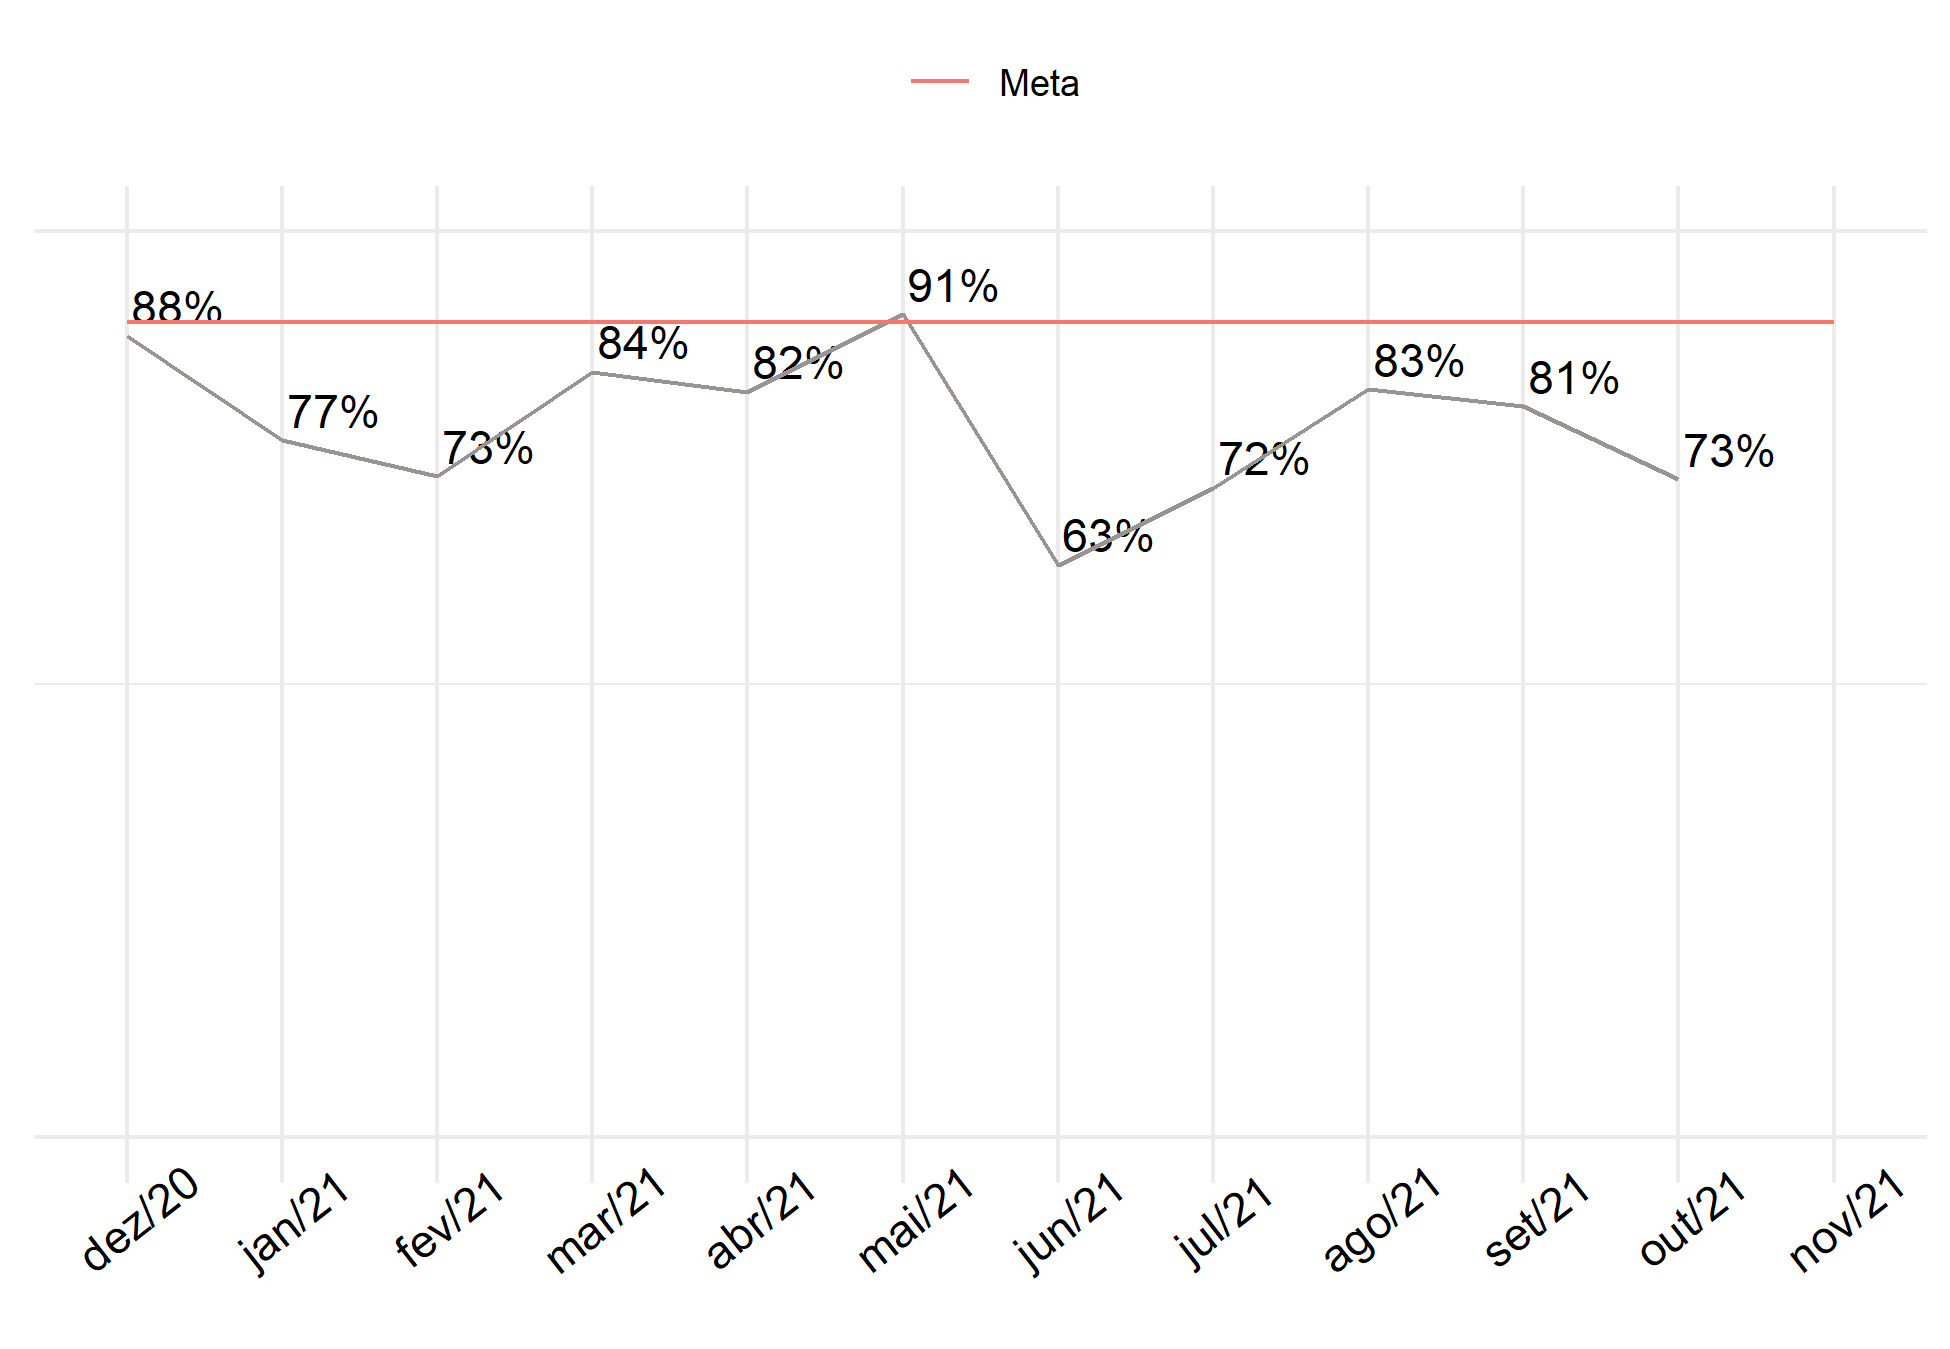
\includegraphics[width=0.7\textwidth]{Imagens/check_alta.png}
\end{figure}

\begin{center}
 \textbf{Meta: 90\%}
\end{center}

\newpage

\subsection{PROTOCOLO DE SEGURANÇA NO USO DE MEDICAMENTOS}

\begin{figure}[H]
\caption{Taxa de erros na prescrição de medicamentos}
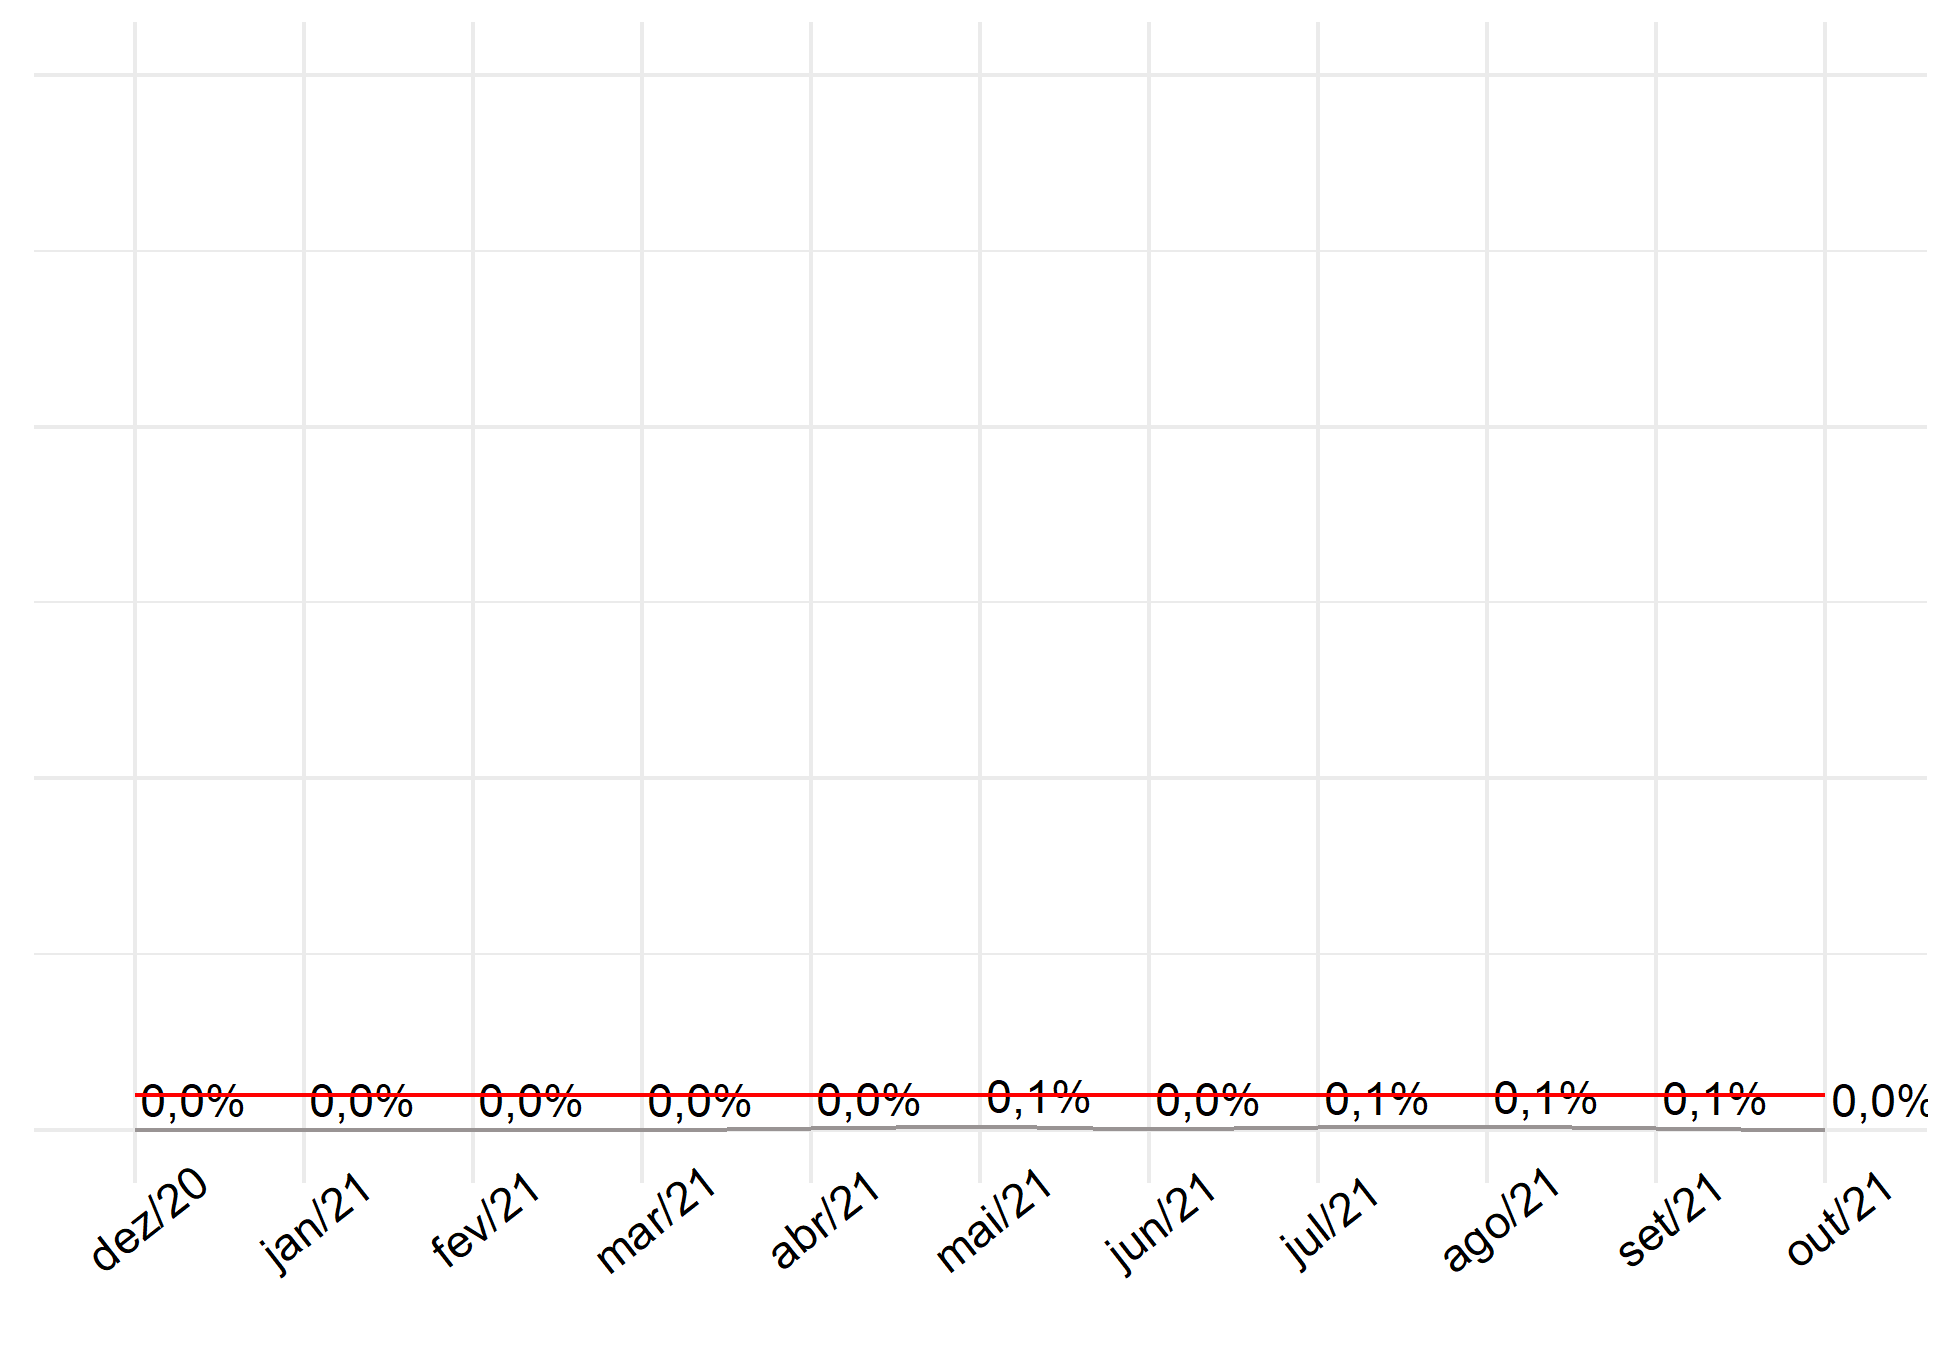
\includegraphics[width=0.7\textwidth]{Imagens/med_prescritos.png}
\end{figure}

\begin{center}
 \textbf{Meta: máximo aceitavel de 1\%}
\end{center}

\begin{figure}[H]
\caption{Taxa de erros na dispensação de medicamentos}
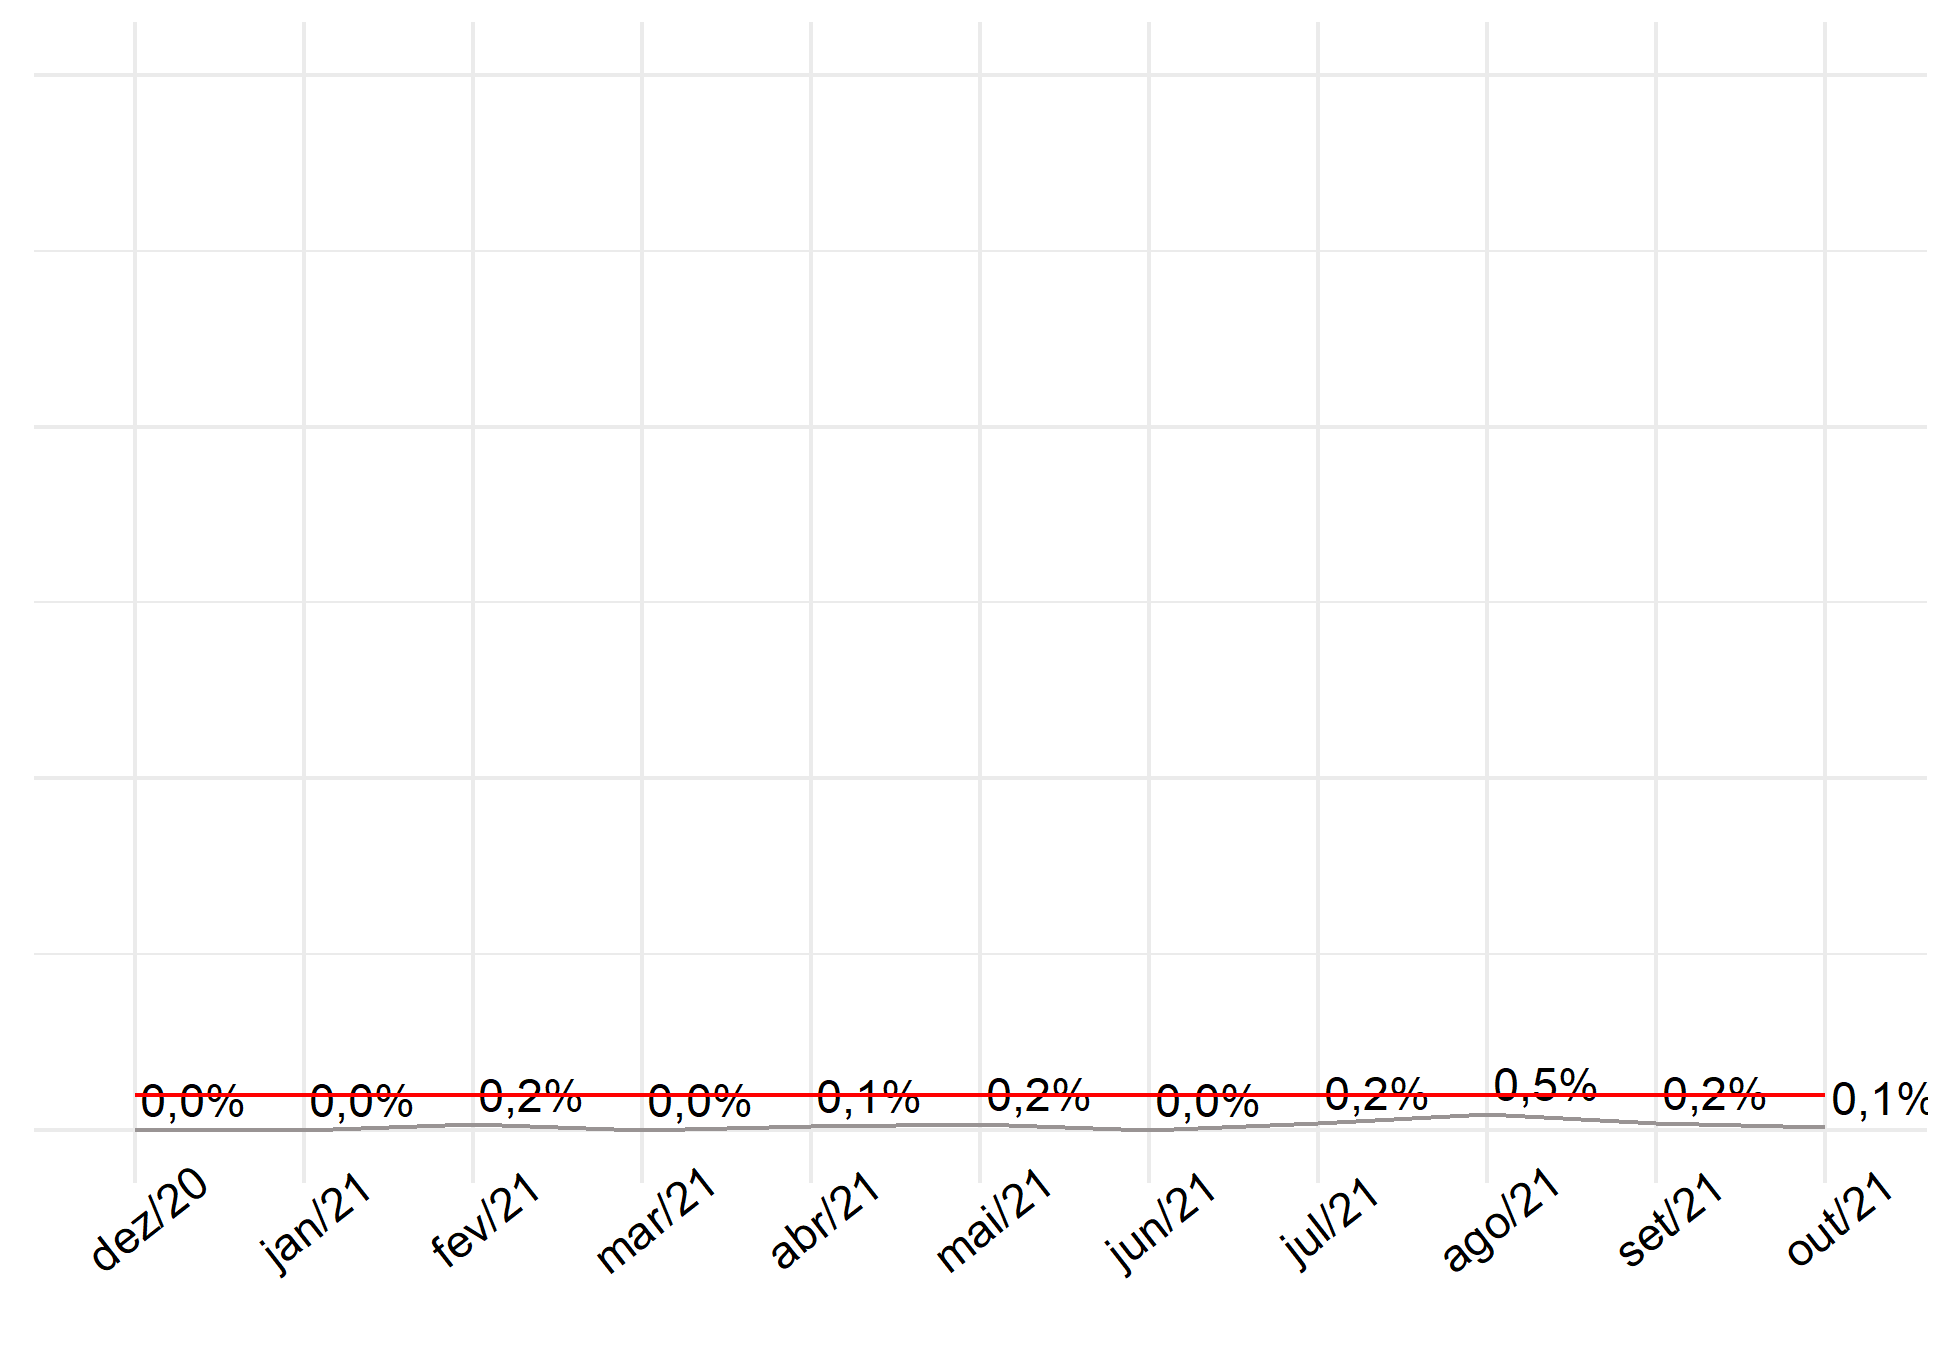
\includegraphics[width=0.7\textwidth]{Imagens/med_dispensados.png}
\end{figure}

\begin{center}
 \textbf{Meta: máximo aceitavel de 1\%}
\end{center}

\newpage

\subsection{PROTOCOLO DE HIGIENIZAÇÃO DAS MÃOS}

\hspace{1cm} A Higienização das Mãos é uma meta internacional
prioritária de segurança, pois é a principal barreira para a transmissão
de infecções relacionadas à assistência.

\hspace{1cm} O Protocolo de Higienização das Mãos integra as
recomendações da RDC nº 36 de 25 de Julho de 2013 e compõe o Anexo 1 da
Portaria 1.377 de 09 de junho de 2013.

\begin{figure}[H]
\caption{Consumo de preparação alcoólica (ml) por paciente-dia}
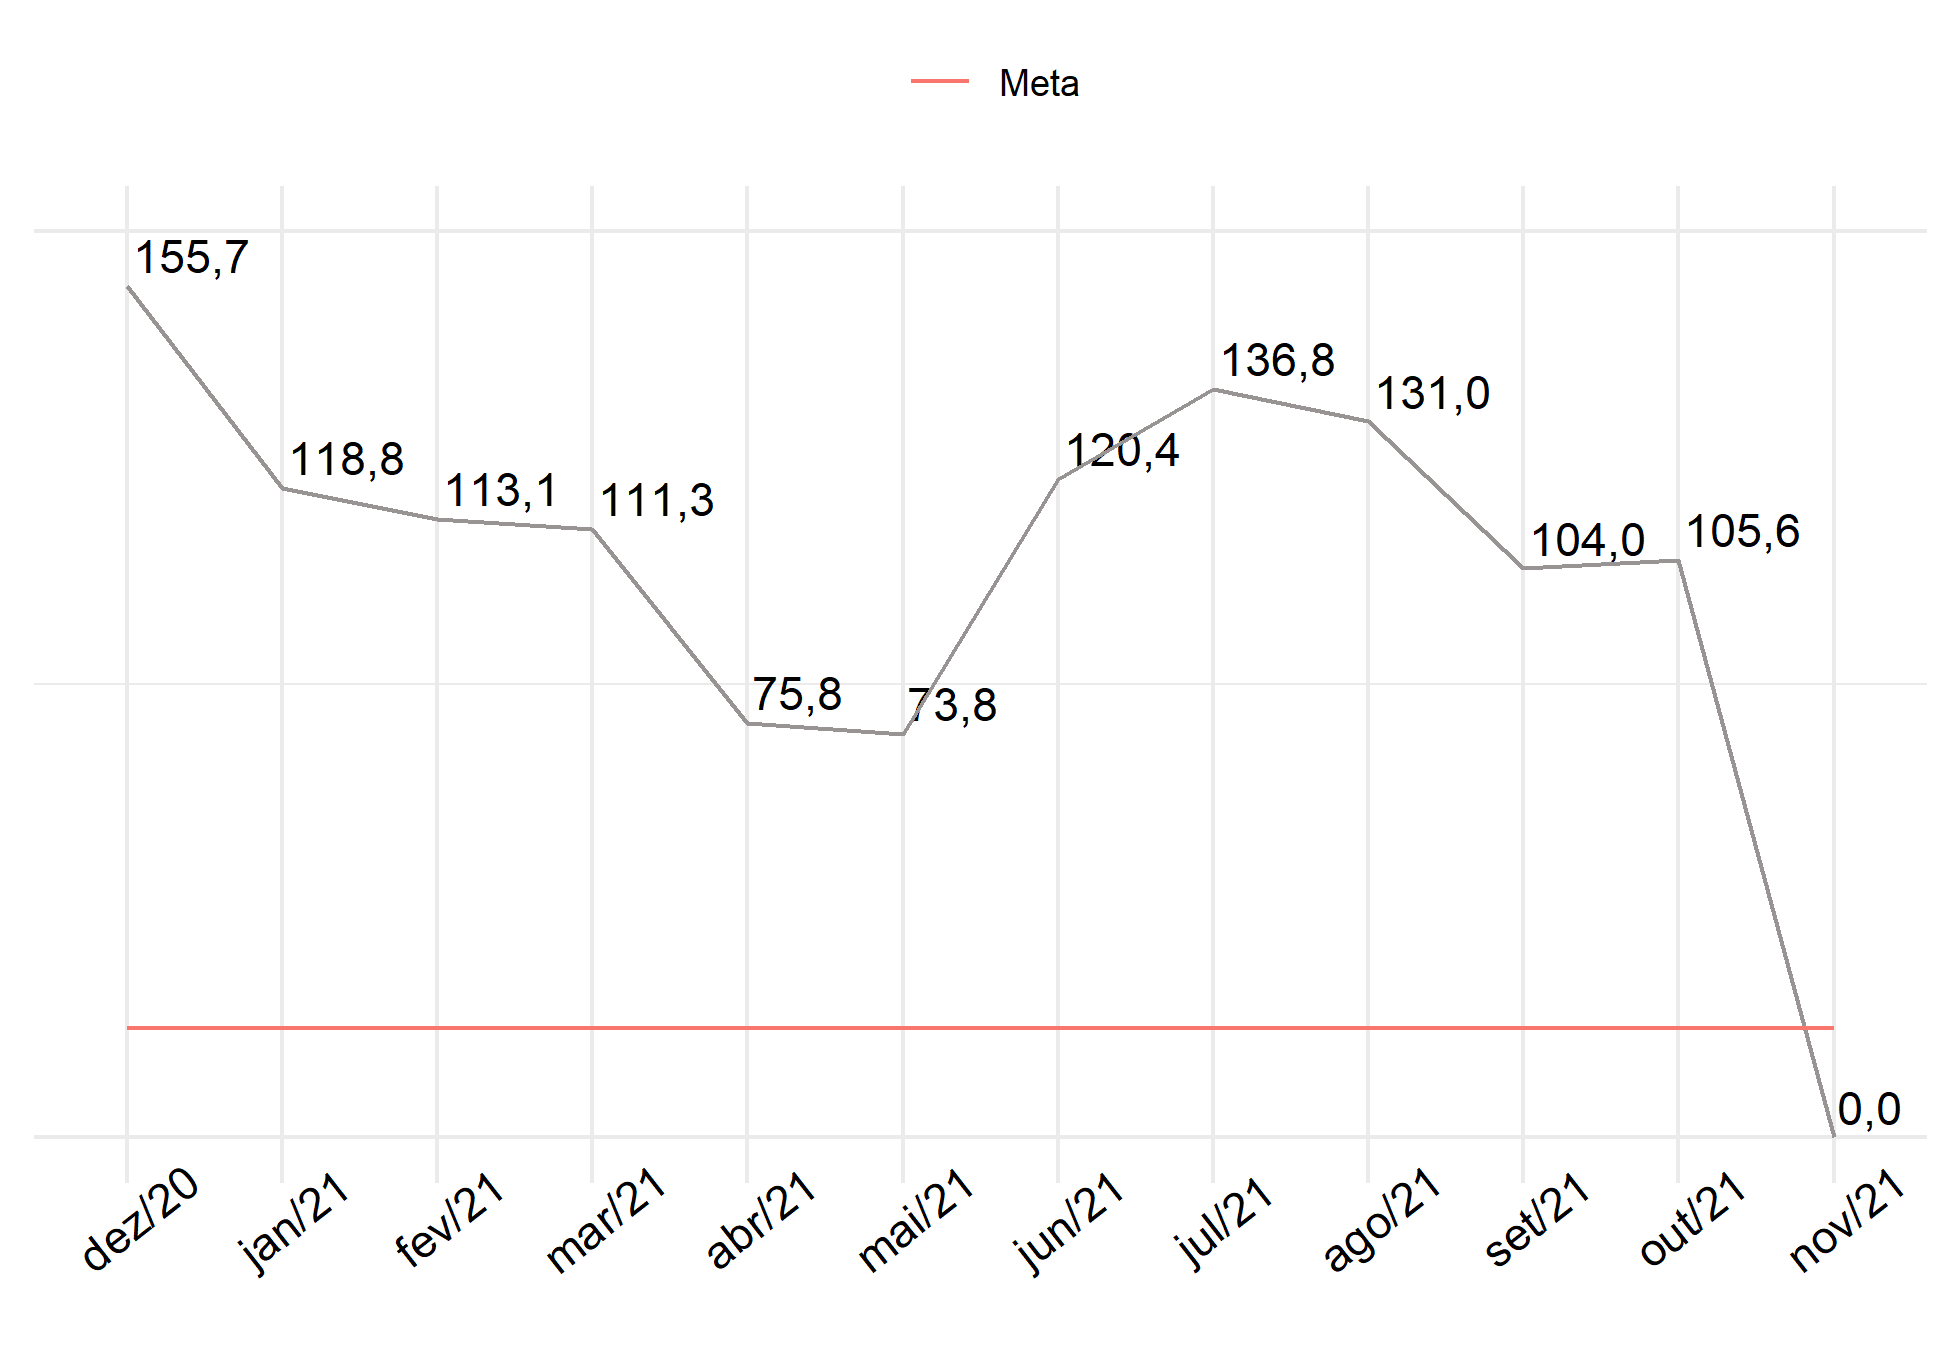
\includegraphics[width=0.7\textwidth]{Imagens/higienizacao_pediatria.png}
\end{figure}

\begin{center}
 \textbf{Meta: 20 ml por paciente-dia}
\end{center}

\subsubsection{CONSIDERAÇÕES}

A higienização das mãos é uma importante barreira na prevenção de
infecções cruzadas. Os Cinco Momentos recomendados pela OMS são:

\begin{enumerate}
    \item Antes do contato com o paciente;
    \item Antes da realização de procedimento asséptico;
    \item O risco de exposição a fluidos corporais;
    \item Contato com o paciente;
    \item Contato com áreas próximas ao paciente.
\end{enumerate}

\fbox{\begin{minipage}{45em}
Lembramos que a técnica correta de higiene de mãos também envolve o tempo (40-60 segundos: água e sabão; 20-30 segundos: preparação alcóolica) e o NÃO USO de adornos.
\end{minipage}}

\newpage
\subsection{PROTOCOLO DE PREVENÇÃO DE QUEDAS}

\begin{figure}[H]
\caption{Taxa de quedas por mil pacientes-dia}
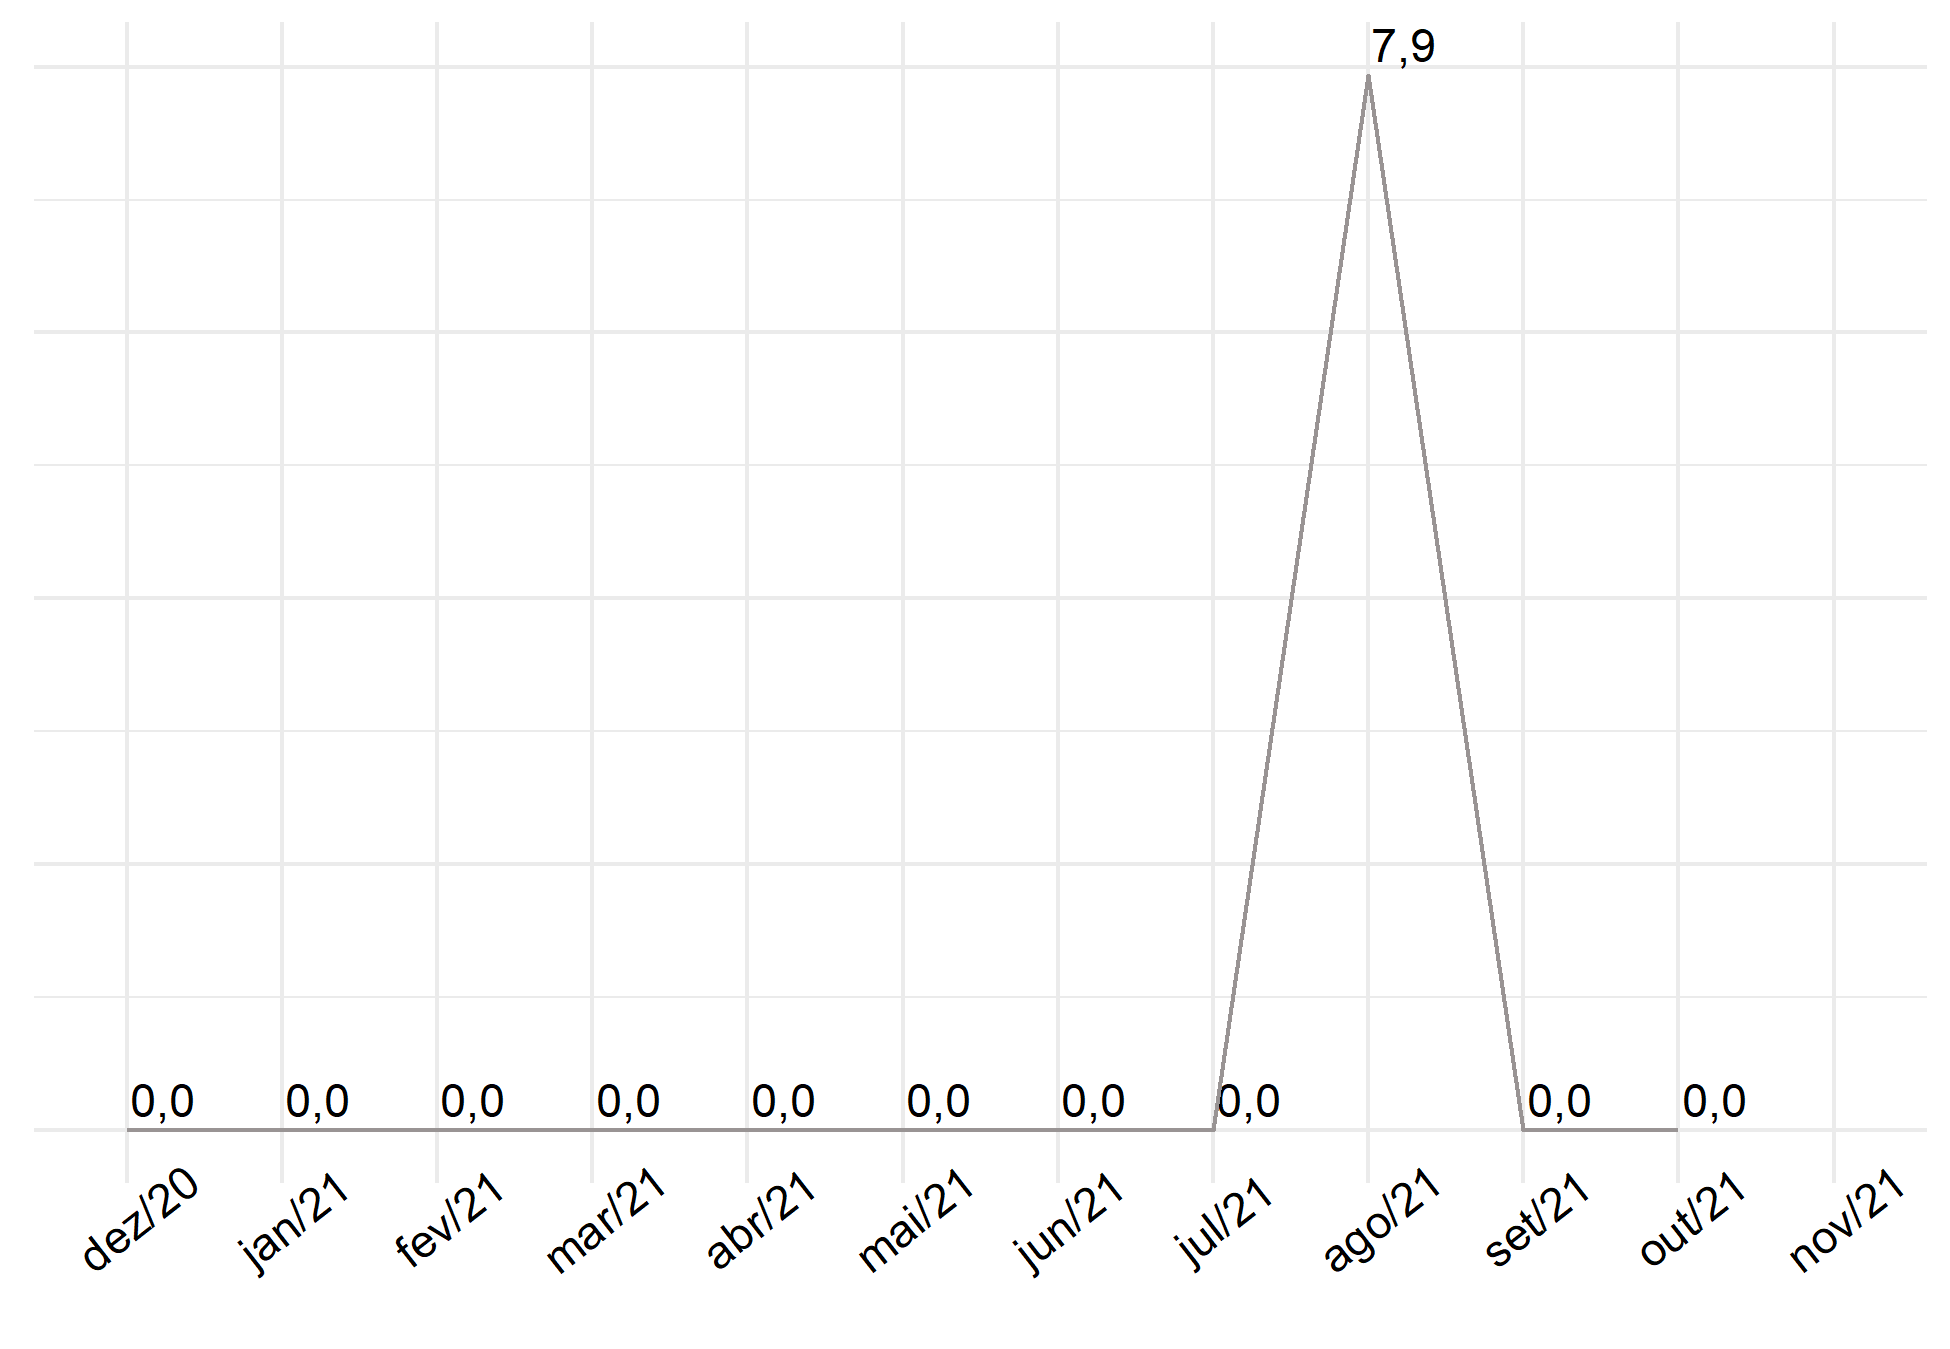
\includegraphics[width=0.7\textwidth]{Imagens/quedas_pacientes_dia.png}
\end{figure}

\begin{figure}[H]
\caption{Taxa de quedas com dano por mil pacientes-dia}
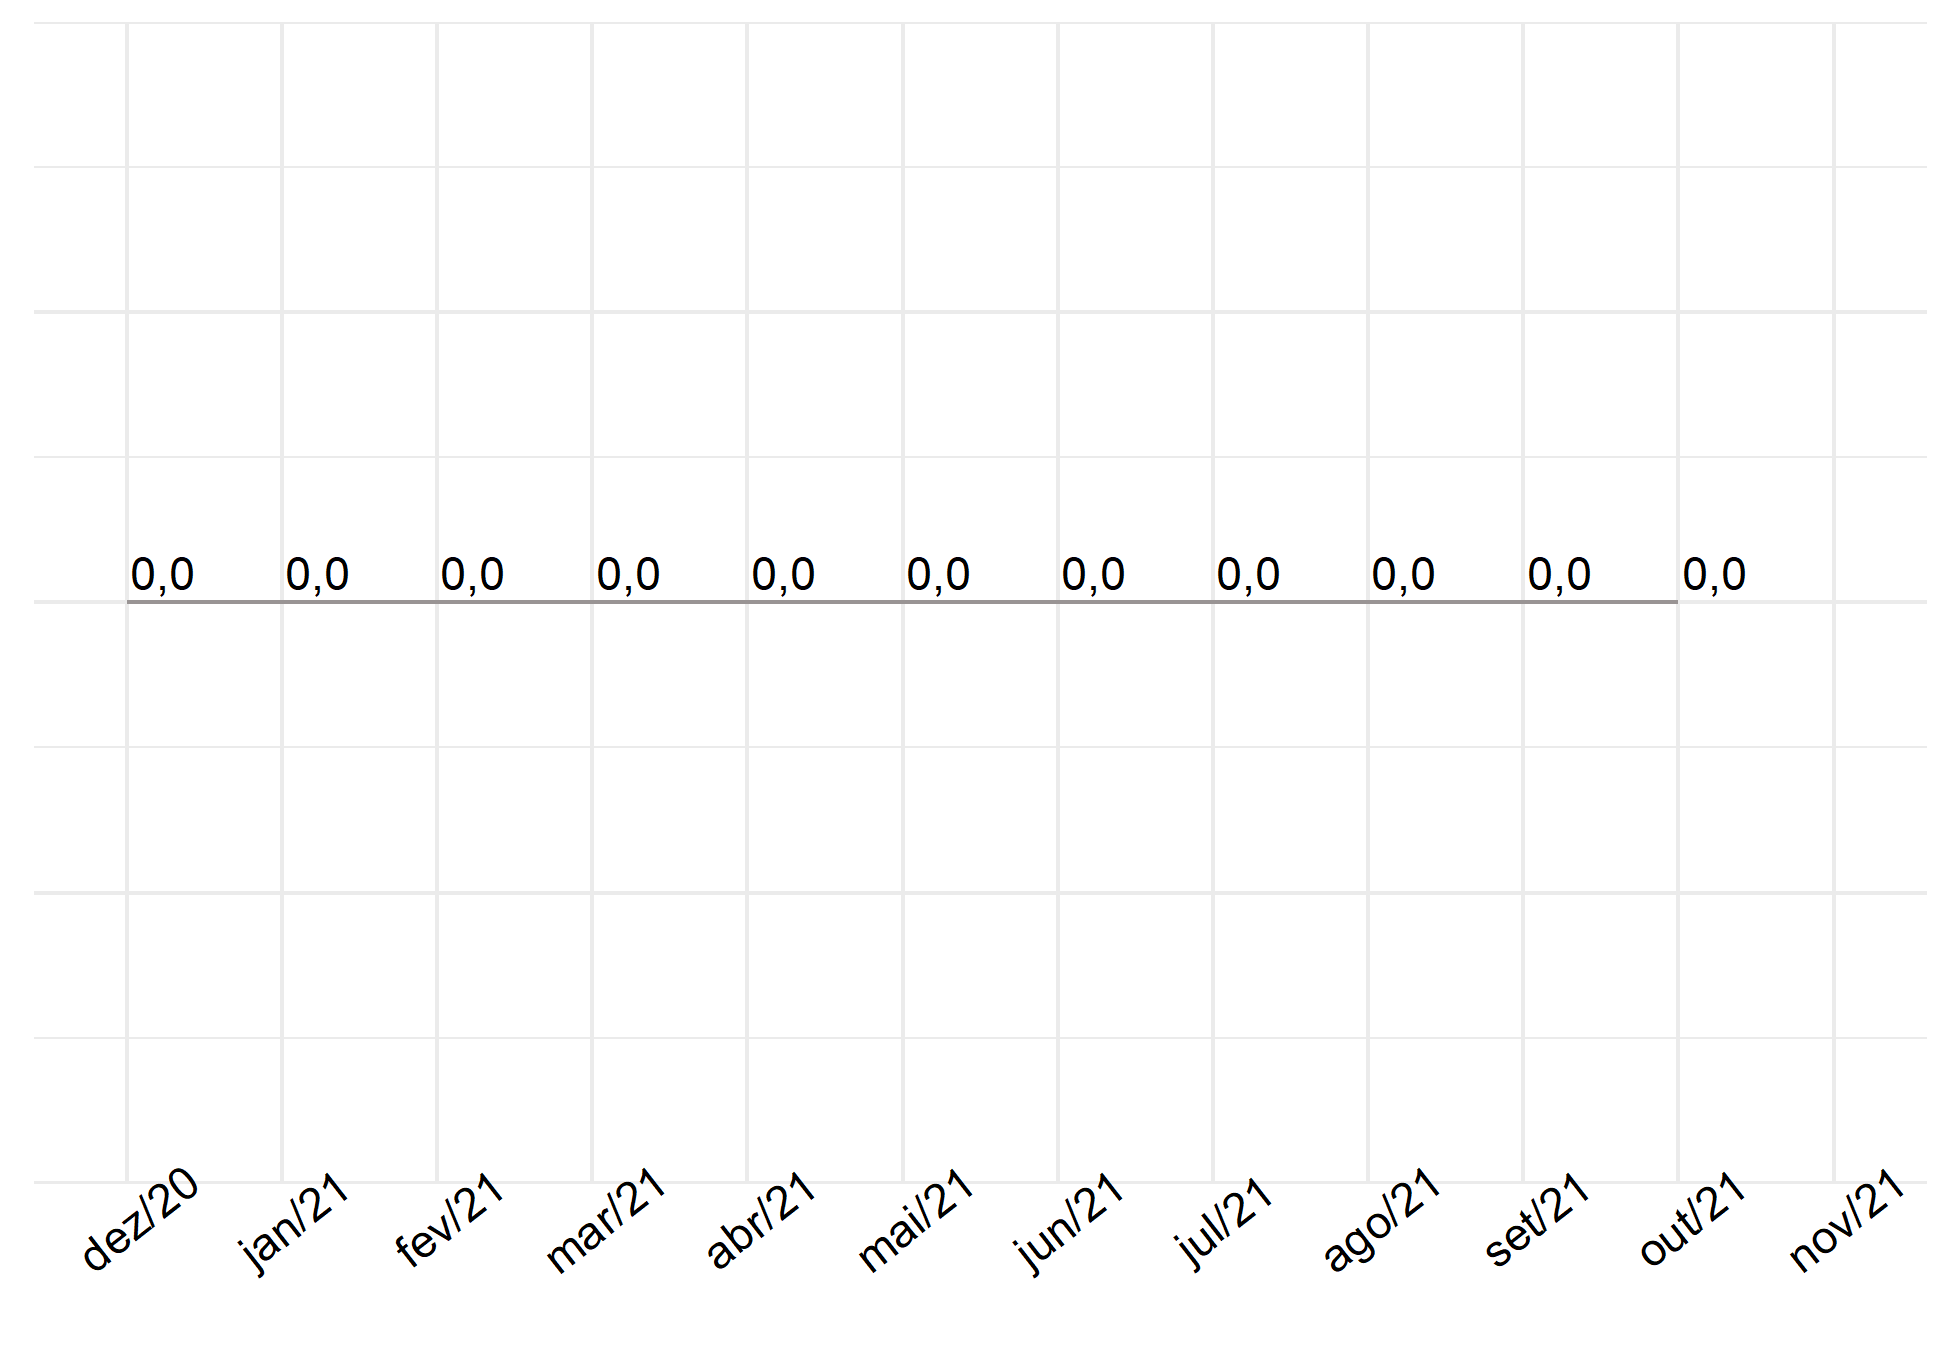
\includegraphics[width=0.7\textwidth]{Imagens/queda_pacientes_dia.png}
\end{figure}

\begin{table}[H]

\caption{\label{tab:unnamed-chunk-15}Distribuição do número de quedas}
\centering
\resizebox{\linewidth}{!}{
\begin{tabular}[t]{lrrrrrrrrrrrrr}
\toprule
 & dez/20 & jan/21 & fev/21 & mar/21 & abr/21 & mai/21 & jun/21 & jul/21 & ago/21 & set/21 & out/21 & nov/21 & Total\\
\midrule
Evento Adverso & 0 & 0 & 0 & 0 & 0 & 0 & 0 & 0 & 0 & 0 & 0 & 0 & 0\\
Incidente sem dano & 0 & 0 & 0 & 0 & 0 & 0 & 0 & 0 & 1 & 0 & 0 & 0 & 1\\
\midrule
\textbf{Total} & \textbf{0} & \textbf{0} & \textbf{0} & \textbf{0} & \textbf{0} & \textbf{0} & \textbf{0} & \textbf{0} & \textbf{1} & \textbf{0} & \textbf{0} & \textbf{0} & \textbf{1}\\
\bottomrule
\end{tabular}}
\end{table}

\newpage 
\subsection{PROTOCOLO DE PREVENÇÃO DE LESÃO POR PRESSÃO}

\begin{figure}[H]
\caption{Percentual de pacientes submetidos à avaliação do risco de lesão por pressão à admissão}
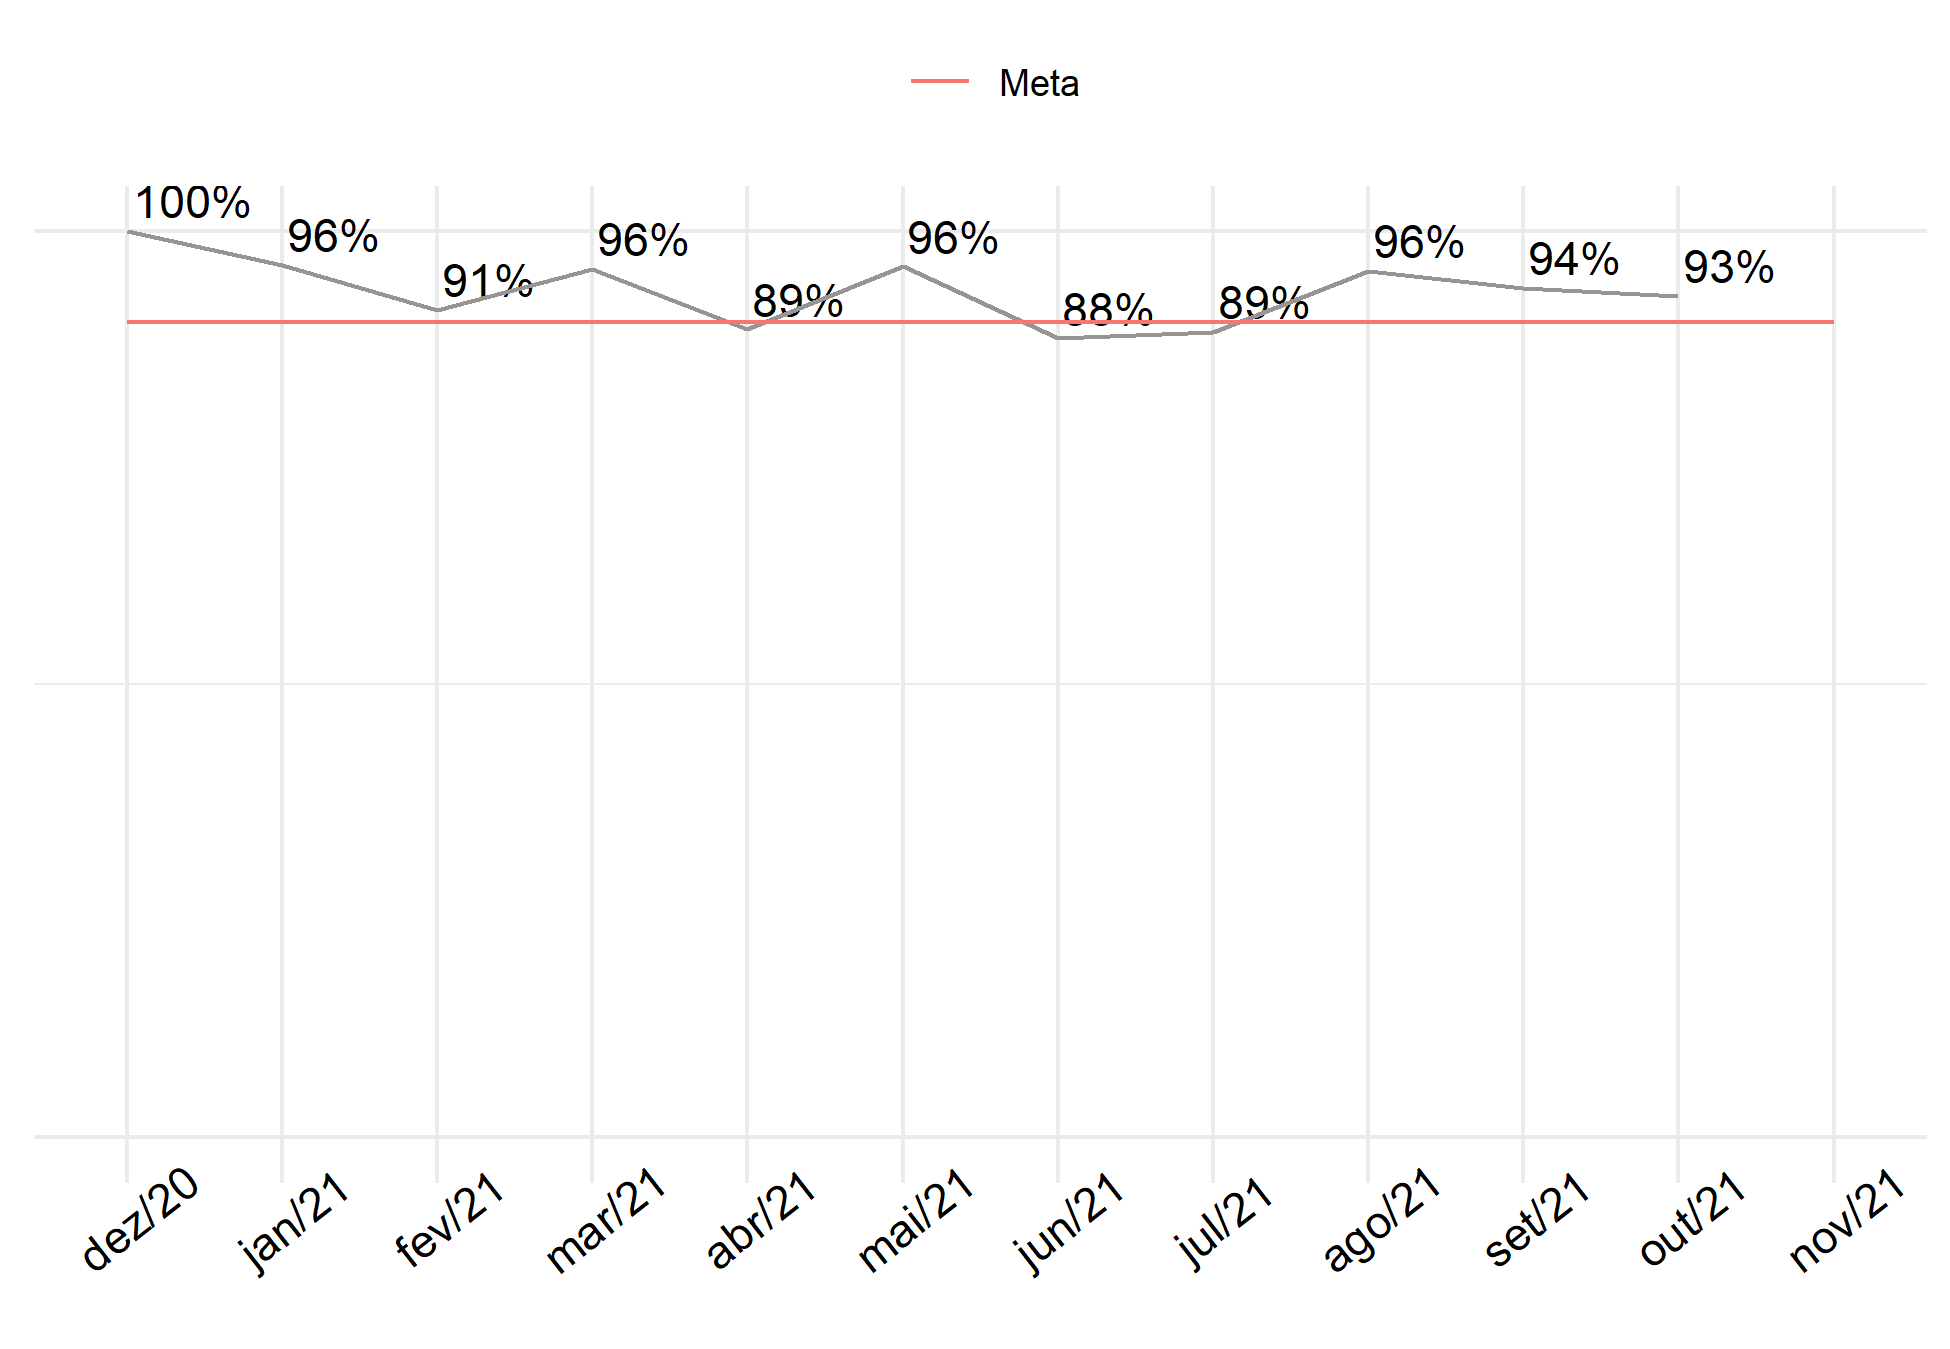
\includegraphics[width=0.7\textwidth]{Imagens/lesao_pressao.png}
\end{figure}

\begin{center}
 \textbf{Meta: 90\%}
\end{center}

\begin{figure}[H]
\caption{Taxa de Lesão por Pressão por mil pacientes-dia}
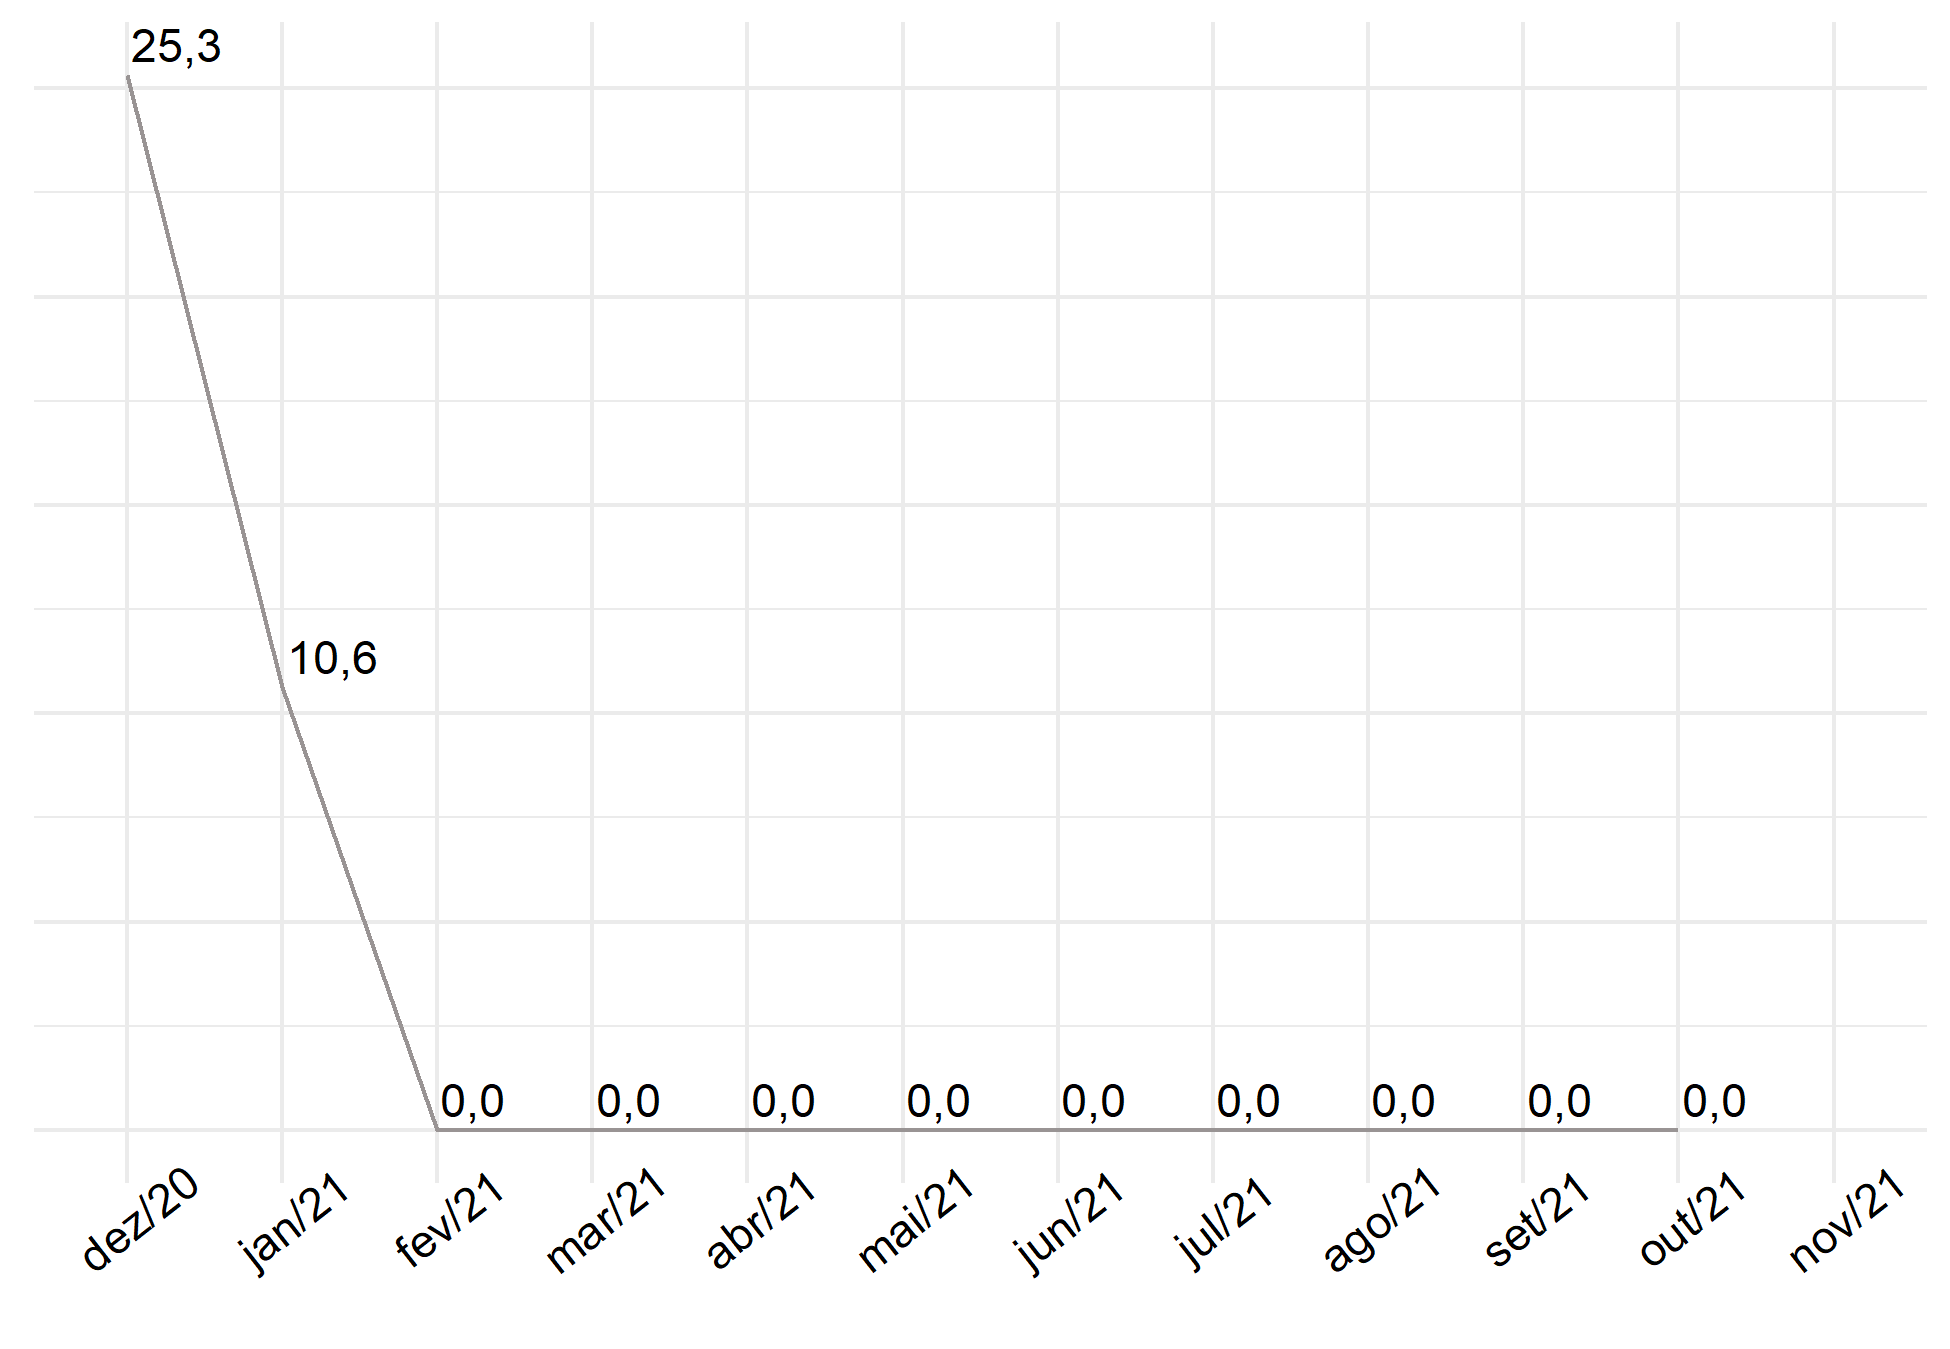
\includegraphics[width=0.7\textwidth]{Imagens/lesaoPressao_pacientes_dia.png}
\end{figure}

\newpage
\subsection{PROTOCOLO DE SEGURANÇA NA TERAPIA NUTRICIONAL ENTERAL}

\begin{table}[H]

\caption{\label{tab:unnamed-chunk-19}Incidência de Perda do CNE nos pacientes em TNE}
\centering
\begin{tabu} to \linewidth {>{\raggedright}X>{\raggedright}X>{\raggedright}X>{\raggedright}X>{\raggedright}X>{\raggedright}X>{\raggedright}X>{\raggedright}X>{\raggedright}X>{\raggedright}X>{\raggedright}X>{\raggedright}X}
\toprule
jan & fev & mar & abr & mai & jun & jul & ago & set & out & nov & dez\\
\midrule
0\% & 0\% & - & 0\% & 0\% & 0\% & 0\% & 0\% & 0\% & 0\% & - & -\\
\bottomrule
\end{tabu}
\end{table}

\begin{table}[H]

\caption{\label{tab:unnamed-chunk-19}Taxa de não conformidade no processo de TNE}
\centering
\begin{tabu} to \linewidth {>{\raggedright}X>{\raggedright}X>{\raggedright}X>{\raggedright}X>{\raggedright}X>{\raggedright}X>{\raggedright}X>{\raggedright}X>{\raggedright}X>{\raggedright}X>{\raggedright}X>{\raggedright}X}
\toprule
jan & fev & mar & abr & mai & jun & jul & ago & set & out & nov & dez\\
\midrule
0\% & 0\% & - & 10\% & 4\% & 0\% & 0\% & 0\% & 0\% & 0\% & - & -\\
\bottomrule
\end{tabu}
\end{table}

\begin{table}[H]

\caption{\label{tab:unnamed-chunk-19}Taxa de pacientes com diarréia recebendo TNE}
\centering
\begin{tabu} to \linewidth {>{\raggedright}X>{\raggedright}X>{\raggedright}X>{\raggedright}X>{\raggedright}X>{\raggedright}X>{\raggedright}X>{\raggedright}X>{\raggedright}X>{\raggedright}X>{\raggedright}X>{\raggedright}X}
\toprule
jan & fev & mar & abr & mai & jun & jul & ago & set & out & nov & dez\\
\midrule
0\% & 0\% & - & 0\% & 0\% & 0\% & 0\% & 0\% & 0\% & 0\% & - & -\\
\bottomrule
\end{tabu}
\end{table}

\begin{table}[H]

\caption{\label{tab:unnamed-chunk-19}Frequência de jejum >48h em pacientes com TNE}
\centering
\begin{tabu} to \linewidth {>{\raggedright}X>{\raggedright}X>{\raggedright}X>{\raggedright}X>{\raggedright}X>{\raggedright}X>{\raggedright}X>{\raggedright}X>{\raggedright}X>{\raggedright}X>{\raggedright}X>{\raggedright}X}
\toprule
jan & fev & mar & abr & mai & jun & jul & ago & set & out & nov & dez\\
\midrule
0\% & 0\% & - & 0\% & 0\% & 0\% & 0\% & 0\% & 0\% & 0\% & - & -\\
\bottomrule
\end{tabu}
\end{table}

\begin{table}[H]

\caption{\label{tab:unnamed-chunk-19}Percentual de pacientes recebendo volume de NE > 70\% do prescrito.}
\centering
\begin{tabu} to \linewidth {>{\raggedright}X>{\raggedright}X>{\raggedright}X>{\raggedright}X>{\raggedright}X>{\raggedright}X>{\raggedright}X>{\raggedright}X>{\raggedright}X>{\raggedright}X>{\raggedright}X>{\raggedright}X}
\toprule
jan & fev & mar & abr & mai & jun & jul & ago & set & out & nov & dez\\
\midrule
100\% & 100\% & - & 100\% & 67\% & 100\% & 100\% & 100\% & 67\% & 83\% & - & -\\
\bottomrule
\end{tabu}
\end{table}

\newpage

\subsection{NOTIFICAÇÃO DE INCIDENTES}

\hspace{1cm} A notificação de incidentes contribui para a gestão de
risco, pois permite o conhecimento dos padrões e semelhanças dos eventos
possibilitando uma intervenção direcionada e objetiva. Nem todo
incidente notificado gera danos ao paciente e, nem todos os incidentes
podem ser evitados. Mas, mediante a notificação, pode-se propor a
revisão dos processos no intento de melhorá-los.

\hspace{1cm} A notificação de incidentes pode ser feita por qualquer
profissional de saúde nos seguintes locais: Sistema de Enfermarias e
Sistema de Informação Hospitalar (SIH) havendo total sigilo do
notificador. As notificações realizadas no ano estão ilustradas abaixo:

\vspace{0.5cm}

\begin{table}[H]

\caption{\label{tab:unnamed-chunk-20}Notificações de Evento Adverso realizadas pelo setor}
\centering
\resizebox{\linewidth}{!}{
\begin{tabular}[t]{lrrrrrrrrrrrrrl}
\toprule
Evento Adverso & dez/20 & jan/21 & fev/21 & mar/21 & abr/21 & mai/21 & jun/21 & jul/21 & ago/21 & set/21 & out/21 & nov/21 & Total & \%\\
\midrule
Lesão por pressão & 2 & 1 & 0 & 0 & 1 & 0 & 1 & 1 & 2 & 0 & 0 & 0 & 8 & 31\%\\
Uso de materiais e artigos para saúde & 0 & 0 & 1 & 1 & 2 & 0 & 0 & 1 & 1 & 1 & 1 & 0 & 8 & 31\%\\
Medicamento & 0 & 0 & 0 & 0 & 1 & 0 & 0 & 0 & 3 & 1 & 1 & 0 & 6 & 23\%\\
Lesão de pele & 0 & 0 & 0 & 1 & 1 & 0 & 0 & 0 & 0 & 0 & 0 & 0 & 2 & 8\%\\
Flebite & 0 & 0 & 0 & 0 & 0 & 1 & 0 & 0 & 0 & 0 & 0 & 0 & 1 & 4\%\\
\addlinespace
Outros incidentes & 0 & 0 & 0 & 0 & 0 & 0 & 0 & 0 & 0 & 1 & 0 & 0 & 1 & 4\%\\
Exames & 0 & 0 & 0 & 0 & 0 & 0 & 0 & 0 & 0 & 0 & 0 & 0 & 0 & 0\%\\
Queda & 0 & 0 & 0 & 0 & 0 & 0 & 0 & 0 & 0 & 0 & 0 & 0 & 0 & 0\%\\
Terapia nutricional & 0 & 0 & 0 & 0 & 0 & 0 & 0 & 0 & 0 & 0 & 0 & 0 & 0 & 0\%\\
Uso de equipamentos & 0 & 0 & 0 & 0 & 0 & 0 & 0 & 0 & 0 & 0 & 0 & 0 & 0 & 0\%\\
\midrule
\addlinespace
\textbf{Total} & \textbf{2} & \textbf{1} & \textbf{1} & \textbf{2} & \textbf{5} & \textbf{1} & \textbf{1} & \textbf{2} & \textbf{6} & \textbf{3} & \textbf{2} & \textbf{0} & \textbf{26} & \textbf{100\%}\\
\bottomrule
\end{tabular}}
\end{table}
\begin{table}[H]

\caption{\label{tab:unnamed-chunk-20}Notificações de Incidente sem dano realizadas pelo setor}
\centering
\resizebox{\linewidth}{!}{
\begin{tabular}[t]{lrrrrrrrrrrrrrl}
\toprule
Incidente sem dano & dez/20 & jan/21 & fev/21 & mar/21 & abr/21 & mai/21 & jun/21 & jul/21 & ago/21 & set/21 & out/21 & nov/21 & Total & \%\\
\midrule
Medicamento & 1 & 1 & 0 & 0 & 2 & 4 & 6 & 1 & 4 & 3 & 2 & 0 & 24 & 51\%\\
Uso de materiais e artigos para saúde & 0 & 0 & 3 & 1 & 0 & 0 & 1 & 1 & 2 & 5 & 2 & 0 & 15 & 32\%\\
Terapia nutricional & 0 & 0 & 0 & 0 & 1 & 1 & 0 & 0 & 0 & 0 & 2 & 0 & 4 & 9\%\\
Exames & 0 & 0 & 0 & 0 & 0 & 1 & 0 & 0 & 0 & 0 & 0 & 0 & 1 & 2\%\\
Outros incidentes & 0 & 0 & 0 & 0 & 0 & 0 & 0 & 0 & 1 & 0 & 0 & 0 & 1 & 2\%\\
\addlinespace
Queda & 0 & 0 & 0 & 0 & 0 & 0 & 0 & 0 & 1 & 0 & 0 & 0 & 1 & 2\%\\
Uso de equipamentos & 0 & 0 & 0 & 0 & 0 & 0 & 0 & 1 & 0 & 0 & 0 & 0 & 1 & 2\%\\
Flebite & 0 & 0 & 0 & 0 & 0 & 0 & 0 & 0 & 0 & 0 & 0 & 0 & 0 & 0\%\\
Lesão de pele & 0 & 0 & 0 & 0 & 0 & 0 & 0 & 0 & 0 & 0 & 0 & 0 & 0 & 0\%\\
Lesão por pressão & 0 & 0 & 0 & 0 & 0 & 0 & 0 & 0 & 0 & 0 & 0 & 0 & 0 & 0\%\\
\midrule
\addlinespace
\textbf{Total} & \textbf{1} & \textbf{1} & \textbf{3} & \textbf{1} & \textbf{3} & \textbf{6} & \textbf{7} & \textbf{3} & \textbf{8} & \textbf{8} & \textbf{6} & \textbf{0} & \textbf{47} & \textbf{100\%}\\
\bottomrule
\end{tabular}}
\end{table}
\begin{table}[H]

\caption{\label{tab:unnamed-chunk-20}Notificações de Quase um erro (Near Miss) realizadas pelo setor}
\centering
\resizebox{\linewidth}{!}{
\begin{tabular}[t]{lrrrrrrrrrrrrrl}
\toprule
Quase um erro (Near Miss) & dez/20 & jan/21 & fev/21 & mar/21 & abr/21 & mai/21 & jun/21 & jul/21 & ago/21 & set/21 & out/21 & nov/21 & Total & \%\\
\midrule
Medicamento & 0 & 0 & 1 & 0 & 1 & 3 & 1 & 5 & 7 & 6 & 1 & 0 & 25 & 89\%\\
Exames & 2 & 0 & 0 & 0 & 0 & 0 & 0 & 0 & 0 & 0 & 0 & 0 & 2 & 7\%\\
Outros incidentes & 0 & 0 & 0 & 0 & 0 & 0 & 0 & 0 & 1 & 0 & 0 & 0 & 1 & 4\%\\
Flebite & 0 & 0 & 0 & 0 & 0 & 0 & 0 & 0 & 0 & 0 & 0 & 0 & 0 & 0\%\\
Lesão de pele & 0 & 0 & 0 & 0 & 0 & 0 & 0 & 0 & 0 & 0 & 0 & 0 & 0 & 0\%\\
\addlinespace
Lesão por pressão & 0 & 0 & 0 & 0 & 0 & 0 & 0 & 0 & 0 & 0 & 0 & 0 & 0 & 0\%\\
Queda & 0 & 0 & 0 & 0 & 0 & 0 & 0 & 0 & 0 & 0 & 0 & 0 & 0 & 0\%\\
Terapia nutricional & 0 & 0 & 0 & 0 & 0 & 0 & 0 & 0 & 0 & 0 & 0 & 0 & 0 & 0\%\\
Uso de equipamentos & 0 & 0 & 0 & 0 & 0 & 0 & 0 & 0 & 0 & 0 & 0 & 0 & 0 & 0\%\\
Uso de materiais e artigos para saúde & 0 & 0 & 0 & 0 & 0 & 0 & 0 & 0 & 0 & 0 & 0 & 0 & 0 & 0\%\\
\midrule
\addlinespace
\textbf{Total} & \textbf{2} & \textbf{0} & \textbf{1} & \textbf{0} & \textbf{1} & \textbf{3} & \textbf{1} & \textbf{5} & \textbf{8} & \textbf{6} & \textbf{1} & \textbf{0} & \textbf{28} & \textbf{100\%}\\
\bottomrule
\end{tabular}}
\end{table}

\end{document}
